\documentclass[a4paper,12pt, titlepage]{report} % размер бумагиё устанавливаем А4, шрифт 12пунктов
\usepackage[T2A]{fontenc}
\usepackage[utf8]{inputenc} % включаем свою кодировку: koi8-r или utf8 в UNIX, cp1251 в Windows
\usepackage[english,russian]{babel} % используем русский и английский языки с переносами
\usepackage{amssymb,amsfonts,amsmath,mathtext,cite,enumerate,float} % подключаем нужные пакеты расширений
\usepackage[dvips]{graphicx} % хотим вставлять в диплом рисунки?
\usepackage{tabularx}
\usepackage{makecell}
% \usepackage{hyperref}
\graphicspath{{figure/}} % путь к рисункам

\makeatletter
\renewcommand{\@biblabel}[1]{#1.} % Заменяем библиографию с квадратных скобок на точку:
\makeatother

% пакет для расположения картинок в ряд
\usepackage{geometry} % Меняем поля страницы
\geometry{left=2.5cm} % левое поле
\geometry{right=1.5cm} % правое поле
\geometry{top=2cm} % верхнее поле
\geometry{bottom=2cm} % нижнее поле

\renewcommand{\theenumi}{\arabic{enumi}.} % Меняем везде перечисления на цифра.цифра
\renewcommand{\labelenumi}{\arabic{enumi}.} % Меняем везде перечисления на цифра.цифра
\renewcommand{\theenumii}{.\arabic{enumii}.} % Меняем везде перечисления на цифра.цифра
\renewcommand{\labelenumii}{\arabic{enumi}.\arabic{enumii}.} % Меняем везде перечисления на цифра.цифра
\renewcommand{\theenumiii}{.\arabic{enumiii}.} % Меняем везде перечисления на цифра.цифра
\renewcommand{\labelenumiii}{\arabic{enumi}.\arabic{enumii}.\arabic{enumiii}.} % Меняем везде перечисления на цифра.цифра

\usepackage[onehalfspacing]{setspace} %"умное" расстояние между строк - установить 1.5 интервала от нормального, эквивалентно

%\usepackage{floatrow} 
\usepackage{indentfirst} % Отделять первую строку раздела абзацным отступом тоже

\newcommand{\empline}{\mbox{}\newline}
\newcommand{\likechapterheading}[1]{
	\begin{center}
		\textbf{\MakeUppercase{#1}}
	\end{center}
}

\usepackage{titlesec}
\titleformat{\chapter}[display]{\filcenter}{\MakeUppercase{\chaptertitlename} \thechapter}{8pt}{\bfseries \MakeUppercase}{}\titleformat{\section}{\normalsize\bfseries}   {\thesection.}{1em}{}\titleformat{\subsection}{\normalsize\bfseries}{\thesubsection.}{1em}{}% Настройка вертикальных и горизонтальных отступов
\titlespacing*{\chapter}{0pt}{-30pt}{8pt}
\titlespacing*{\section}{\parindent}{*4}{*1}
\titlespacing*{\subsection}{\parindent}{*4}{*1}

\makeatletter
\renewcommand{\@dotsep}{2}\newcommand{\l@likechapter}[2]{{\bfseries\@dottedtocline{1}{0pt}{0pt}{#1}{#2} }} \makeatother \newcommand{\likechapter}[1]{
\newpage \clearpage \likechapterheading{#1}

\addcontentsline{toc}{likechapter}{\MakeUppercase{#1}}}

\usepackage{tocloft}
\renewcommand\contentsname{Содержание}
\renewcommand{\cfttoctitlefont}{\newpage\hspace{0.38\textwidth}\bfseries\MakeUppercase } % Оформление надписи Оглавление
\renewcommand{\cftbeforetoctitleskip}{-1em}
%\renewcommand{\cftaftertoctitle}{\mbox{}\hfill \\ \mbox{}\hfill{\footnotesize Стр.}\vspace{-2.5em}} % Добавим надпись стр.
\renewcommand{\cftchapleader}{\cftdotfill{\cftdotsep}} % Отточия после глав
\renewcommand{\cftchapaftersnum}{.} % Точка после номера главы
\renewcommand{\cftsecaftersnum}{.} % Точка после номера параграфа

\renewcommand{\cftchapfont}{\normalsize\bfseries \MakeUppercase{\chaptername} } % Оформления надписи Глава
\renewcommand{\cftsecfont}{\hspace{31pt}} % Сдвиг названия секции от левого края
\renewcommand{\cftsubsecfont}{\hspace{1pt}}
\renewcommand{\cftbeforechapskip}{1em}
\renewcommand{\cftparskip}{-1mm}  
\renewcommand{\cftdotsep}{1} \setcounter{tocdepth}{1} % Задать глубину оглавления — до subsection включительно

% Оформление подписи к рисункам и таблицам
\usepackage[font=small, tableposition=top]{caption}
\usepackage{subcaption}
\DeclareCaptionLabelFormat{gostfigure}{Рисунок #2}
\DeclareCaptionLabelFormat{gosttable}{Таблица #2}
\DeclareCaptionLabelSeparator{gost}{. }
\captionsetup{labelsep=gost}
\captionsetup[figure]{labelformat=gostfigure}
\captionsetup[table]{labelformat=gosttable}
\renewcommand{\thesubfigure}{\asbuk{subfigure}}

\usepackage[title,titletoc]{appendix}
\titleformat{\paragraph}[display]{\filcenter}{\MakeUppercase{\chaptertitlename} \thechapter}{8pt}{\bfseries}{}
\titlespacing*{\paragraph}{0pt}{-30pt}{8pt}
\newcommand{\append}[1]{\clearpage
\stepcounter{chapter}
\paragraph{\MakeUppercase{#1}}
\empline     \addcontentsline{toc}{likechapter}{\MakeUppercase{\chaptertitlename~\Asbuk{chapter}.\;#1}}}

\bibliographystyle{utf8gost705u}
%\usepackage[nottoc,notlot,notlof]{tocbibind}
\usepackage[square,numbers,sort&compress]{natbib}
\renewcommand{\bibnumfmt}[1]{#1.\hfill} % нумерация источников в самом списке — через точку
\renewcommand{\bibsection}{\likechapter{Список литературы}} % заголовок специального раздела
\setlength{\bibsep}{0pt}

\usepackage{listings}
\usepackage{color}
\usepackage{xcolor}


\lstdefinestyle{customc}{
  belowcaptionskip=1\baselineskip,
  breaklines=true,
  frame=L,
  xleftmargin=\parindent,
  showstringspaces=false,
  basicstyle=\footnotesize\ttfamily,
  keywordstyle=\bfseries\color{green!40!black},
  commentstyle=\itshape\color{purple!40!black},
  identifierstyle=\color{blue},
  stringstyle=\color{orange},
  numbers=left,               % где поставить нумерацию строк (слева\справа)
  numberstyle=\tiny  
}

\lstdefinestyle{customasm}{
  belowcaptionskip=1\baselineskip,
  frame=L,
  xleftmargin=\parindent,
  language=[x86masm]Assembler,
  basicstyle=\footnotesize\ttfamily,
  commentstyle=\itshape\color{purple!40!black},
}

\lstset{escapechar=@,style=customc}

\usepackage[utf8]{inputenc}%включаем свою кодировку: koi8-r или utf8 в UNIX, cp1251 в Windows

\usepackage{enumitem}
\makeatletter
\AddEnumerateCounter{\asbuk}{\@asbuk}{м)}
\makeatother
\setlist{nolistsep}
\renewcommand{\labelitemi}{-}
\renewcommand{\labelenumi}{\asbuk{enumi})}
\renewcommand{\labelenumii}{\arabic{enumii})}

\usepackage{amsthm}
\theoremstyle{plain}
\newtheorem{thm}{Theorem}[section]
%\newtheorem{thm}{Theorem}[subsection]
%\newtheorem{defn}[thm]{Definition}
\newtheorem{St}{Утверждение}
\newtheorem{Th}{Теорема}
\newtheorem{Cor}{Следствие}
\newtheorem{Lm}{Лемма}

\begin{document}
	\singlespacing % Одинарный междустрочный интервал
	\begin{titlepage}
	\newpage
	\begin{center}
		
\includegraphics[width=0.8cm]{logo_unn_crop.eps} \\
		МИНИСТЕРСТВО  НАУКИ И ВЫСШЕГО ОБРАЗОВАНИЯ \\ 
		РОССИЙСКОЙ  ФЕДЕРАЦИИ  \\
		%\vspace{1cm}
		Федеральное государственное автономное образовательное учреждение\\* высшего образования \\*
		\textbf{<<Национальный исследовательский \\* Нижегородский государственный университет им. Н.И. Лобачевского>>}\\*
		\textbf{(ННГУ)}\\*
		\vspace{2em}
		\textbf{Институт информационных технологий, математики и механики}\\*
		\textbf{Кафедра: Теории управления и динамики систем}\\*
		\vspace{2em}
		Направление подготовки: <<Фундаментальная информатика и информационные технологии>>\\*
		Профиль подготовки: <<Когнитивные системы>>\\*
	\end{center}

	\vspace{1em}

	\begin{center}
		{\Large \textbf{ОТЧЕТ ПО УЧЕБНОЙ ПРАКТИКЕ}}
    \end{center}

    \vspace{2.5em}

	\begin{center}
		{\textbf{На тему:}}\\
		
		{\large \textbf{<<Двухкластерные режимы в системе Курамото с инерцией>>}}
	\end{center}

    \vspace{4em}

    \hfill
    \begin{minipage}[t]{.36\linewidth}
    	\begin{flushleft}
    	
			\textbf{Выполнил(а):} студент(ка) группы 382006-3м \\
			% \vspace{1.0em}
			Хорькин Дмитрий Сергеевич\\
			\vspace{1.0em}
			\hrulefill  \\
			{\small подпись}\\
			
			\vspace{1.5em}
			\textbf{Научный руководитель:}\\
		доцент, к.ф.-м.н.\\
			% \vspace{1.0em}
			Смирнов Лев Александрович\\
			\vspace{1.0em}
			\hrulefill  \\
			{\small подпись}
			
    	\end{flushleft}
    \end{minipage}

	\vspace{\fill}

	\begin{center}
		Нижний Новгород \\
		2022
	\end{center}

\end{titlepage} % Это титульный лист
	\setcounter{page}{2} % Нумерация страниц со 2-й, 1-й является титульная страница
	\onehalfspacing % Полуторный междустрочный интервал
	\setlength{\parindent}{1.25cm} % Абзацный отступ

	\likechapter{Аннотация}
В данной работе рассматриваются двухкластерные вращательные режимы в системе Курамото с инерцией. 
В частности, изучается вопрос существования и устойчивости двухкластерных вращательных режимов в зависимости от управляющий параметров.
Также был реализован программный комплекс, позволяющий эффективно находить интересующие вращательные
режимы в произвольных системах связанных элементов.
Было разработано web-приложение, выполняющее прямое численное моделирование системы.
Аналитические результаты подтверждены прямым численным моделированием.

	\def\contentsname{Содержание} % "Содержание" вместо "Оглавление"
	\def\bibname{Список литературы}
	\tableofcontents % Это оглавление, которое генерируется автоматически
	\likechapter{Введение}
Сети фазовых осцилляторов часто используются для моделирования
совместной динамики в различных биологических и
искусственных системах, начиная от нейронных сетей \cite{Hoppensteadt:Izhikevich} и
популяций химических осцилляторов \cite{Tinsley:Nkomo} до лазерных решеток \cite{Ding:Belykh}
и электрических сетей \cite{Dorfler:Chertkov}. Система
фазовых осцилляторов Курамото первого порядка \cite{Kuramoto,Strogatz} представляет собой широко адаптированную модель
сети фазовых осцилляторов, которая может демонстрировать сложную
пространственно-временную динамику при переходе от
некогерентности к полной синхронизации \cite{Acebron:Bonilla,Barreto:Hunt,Ott:Antonsen,Hong:Chate,Pikovsky:Rosenblum,Maistrenko:Popovych,Dorfler:Bullo,Martens:Barreto}.
Когда колебания в модели Курамото имеют неоднородные частоты, этот переход обычно
сопровождается частичной синхронизацией, которая возникает, когда система
распадается на кластеры когерентных и некогерентных осцилляторов
\cite{Acebron:Bonilla,Martens:Barreto,Laing}.

Модель Курамото второго порядка с инерцией обычно используется для описания сетей генераторов,
способных регулировать свои собственные частоты, как, например, в адаптивной частотной
модели синхронизации светлячков \cite{Ermentrout} и системах электросетей \cite{Tumash}.
Включение инерции приводит к двумерной внутренней динамике осциллятора,
тем самым делая кооперативную динамику модели Курамото второго порядка существенно более
сложной, чем ее классическая противоположная часть первого порядка.
Эта динамика, вызванная инерцией, включает сложные переходы от некогерентности
к полной синхронизации \cite{Tanaka:Review,Tanaka:Physica,Peron,Munyaev:Smirnov,Komarov:Gupta,Olmi:Navas,Barabash:Belykh},
бистабильность синхронных кластеров \cite{Belykh:Brister}, хаотическую межкластерную динамику \cite{Brister:Belykh},
химеры \cite{Olmi:Chaos, Maistrenko:Brezetsky, Medvedev:Mizuhara} и уединенные состояния \cite{Jaros:Maistrenko, Jaros:Brezetsky}.

В работе \cite{Belykh:Brister} аналитически изучили возникновение и сосуществование стабильных
кластеров в двухпопуляционной сети идентичных осцилляторов Курамото второго порядка.
Две популяции разных размеров $K$ и $M$ естественным образом разделились бы на два кластера,
где осцилляторы синхронизируются внутри кластера, создавая фазовый сдвиг между кластерами.
Анализ, выполненный в \cite{Belykh:Brister}, позволил получить необходимые и достаточные условия для стабильности
двухкластерной синхронизации с постоянной фазой, а
также предоставил условие устойчивости концепции для двухкластерной синхронизации с
вращающимся фазовым сдвигом. 

Целью данной работы является изучение двухкластерных вращательных режимов в системе Курамото
с инерцией и запаздывающей по фазе связью Курамото-Сакагути, для успешного достижения которой выделены следующие задачи: \\
1) Исследование существования и типов возникающих двухкластерных вращательных режимов в зависимости от управляющих параметров. \\
2) Исследование устойчивости двухкластерных вращательных режимов в зависимости от управляющих параметров. \\
3) Реализация программного комплекса, позволяющего эффективно находить интересующие вращательные движения, а также определять
их устойчивость в произвольных системах связанных элементов.

	\begin{chapter}{Модель Курамото. Двухкластерные вращательные режимы}
	\section{Модель Курамото с инерцией}
	В данной работе исследуется модель Курамото второго порядка, описываемая системой уравнений:
	\begin{equation} \label{main-sistem}
		m\ddot{\varphi}_i + \dot{\varphi}_i = \omega + 
		\frac{1}{N} \sum_{j = 1}^N \sin{(\varphi_j - 
		\varphi_i - \alpha)}, i = \overline{1, N}, 
	\end{equation}
	где $m$ - параметр инерции, $\omega$ - постоянный вращающий момент,
	$\alpha$ - фазовая задержка, $N$ - общее число элементов.
	Предполагается, что осцилляторы являются идентичными, с идентичной частотой $\omega$, массой $m$ и запаздыванием по
	фазе $\alpha \in [0, \pi)$ \cite{Sakaguchi} . В системе \eqref{main-sistem} имеется синфазный режим,
	который локально устойчив для любого $\alpha \in [0, \pi/2)$
	и нестабилен для любого $\alpha \in [\pi/2, \pi)$ \cite{Acebron:Bonilla}. Поэтому принято считать связь притягивающей при
	$\alpha < \pi/2$ и отталкивающей при $\pi/2 \leq \alpha < \pi$.

	\section{Двухкластерные вращательные режимы. Существование и типы}
	
	Заметим, что двухкластерный режим описывается системой:
	
	\begin{equation} \label{two-cluster}
		\begin{cases}
			m\ddot{\psi}_1 + \dot{\psi}_1 = \omega + \frac{N-K}{N} \sin{(\psi_2 - \psi_1 - \alpha)} - \frac{K}{N}\sin{\alpha},\\
			m\ddot{\psi}_2 + \dot{\psi}_2 = \omega + \frac{K}{N} \sin{(\psi_1 - \psi_2 - \alpha)} - \frac{N - K}{N}\sin{\alpha},
		\end{cases}
	\end{equation}
	где $\psi_1$, $\psi_2$ - фазы элементов первого и
	второго кластера соответственно, $K$ - количество элементов в малом кластере.
	Введем новую переменную $\beta = \frac{K}{N}$, характеризующую долю элементов малого кластера относительно размера $N$ всего ансамбля.
	Уравнение \eqref{two-cluster} перепишется в виде:
	
	\begin{equation} \label{two-cluster-beta}
		\begin{cases}
			m\ddot{\psi}_1 + \dot{\psi}_1 = \omega + (1 - \beta) \sin{(\psi_2 - \psi_1 - \alpha)} - \beta\sin{\alpha}, \\
			m\ddot{\psi}_2 + \dot{\psi}_2 = \omega + \beta \sin{(\psi_1 - \psi_2 - \alpha)} - (1 - \beta)\sin{\alpha}.
		\end{cases}
	\end{equation}
	
	Введем величину $X = \psi_1 - \psi_2$, характеризующую расстройку фаз между элементами двух кластеров.
	Вычитая в \eqref{two-cluster-beta} из первого уравнения второе, приходим к уравнению для отстройки $X$:

	\begin{equation} \label{pre-pend}
		m\ddot{X} + \dot{X} = (1 - 2 \beta) \sin{\alpha} - \left[(1-\beta)\sin{(X + \alpha)} + \beta\sin{(X - \alpha)} \right].
	\end{equation}
	
	Заметим, что решение $X = 0$ соответствует реализации
	синфазного вращательного режима. Ненулевое решение $X \neq 0$ соответствует
	реализации двухкластерного режима.
	
	
	Для дальнейшего анализа уравнения \eqref{pre-pend} произведем ряд замен, а именно:
	\begin{align*}
	R^2 = (N - 2K)^2 \sin{\alpha}^2 + N^2 \cos{\alpha}^2, \\
	\rho = \sqrt{\frac{N}{m R}}, \ t = \hat{t} \frac{N}{\rho R}, \gamma = \frac{N - 2K}{R}\sin{\alpha}, \\
	\Phi = X + \delta, \ \delta = \arccos{(\frac{N}{R}\cos{\alpha})}, \\
	\end{align*}
	что приводит к:
	
	\begin{equation} \label{pend}
		\frac{d^2 \Phi }{d\hat{t}^2} + \rho \frac{d\Phi}{d\hat{t}} + \sin{\Phi} = \gamma.
	\end{equation}

	\begin{figure}[h!]
		\begin{center}
			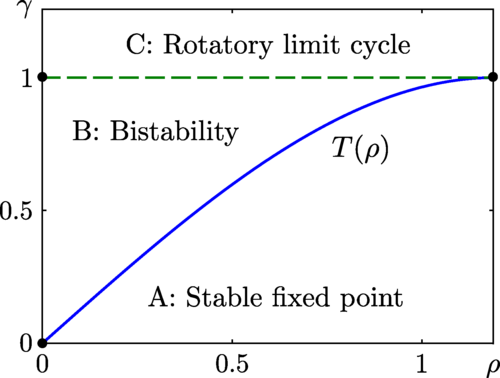
\includegraphics[width=0.7\columnwidth]{pictures/bf-tricommy.png}
		\end{center}
		\caption{Бифуркационная диаграмма нелинейного осциллятора}
		\label{bf-d}
	\end{figure}

	Полученное уравнение \eqref{pend} хорошо изучено в работе \cite{Andronov:Vitt}.
	В зависимости от параметров $\rho$ и $\gamma$, в системе \eqref{pend}
	могут существовать два состояния равновесия:
	устойчивая точка $\Phi_e = \arcsin{\gamma}$ и седло
	$\Phi_s = \pi - \arcsin{\gamma}$, а также
	некоторое устойчивое периодическое вращательное движение.
	Данные соотношения определяются так называемой
	бифуркационной кривой Трикомми (см. рис. \ref{bf-d}).
	Таким образом, в исходной системе могут существовать 2 типа
	двухкластерных вращательных режимов, первый характеризуется
	постоянной расстройкой фаз, второй характеризуется
    периодической на цилиндре расстройкой фаз.
	Область существования вращательного движения в уравнении \eqref{pend}
	определяется соотношением:
	\begin{equation}
		\gamma \ge T(\rho),
	\end{equation}
	где $T(.)$ - уравнение кривой Трикомми. В качестве аппроксимации для кривой Трикоми можно использовать выражение
	$T(\rho) = \rho\frac{4}{\pi} - 0.305\rho^3$ полученное в \cite{Belykh:Brister}.
	Подставляя, получаем уравнения для границы области существования двухкластерного вращательного движения с
	периодической расстройкой фаз в области параметров $\alpha$, $m$:
	\begin{equation} \label{borders}
		m = \frac{1}{\sqrt{(1 - 2\beta)^2\sin{\alpha}^2 + \cos{\alpha}^2} \cdot T^{-1}(\frac{(1 - 2\beta)\sin{\alpha}}{\sqrt{(1 - 2\beta)^2\sin{\alpha}^2 + \cos{\alpha}^2}})}.
	\end{equation}

	Заметим, что двухкластерный вращательный режим при $\beta = 0.5$ не существует.

	\begin{figure}[h!]
		\begin{center}
			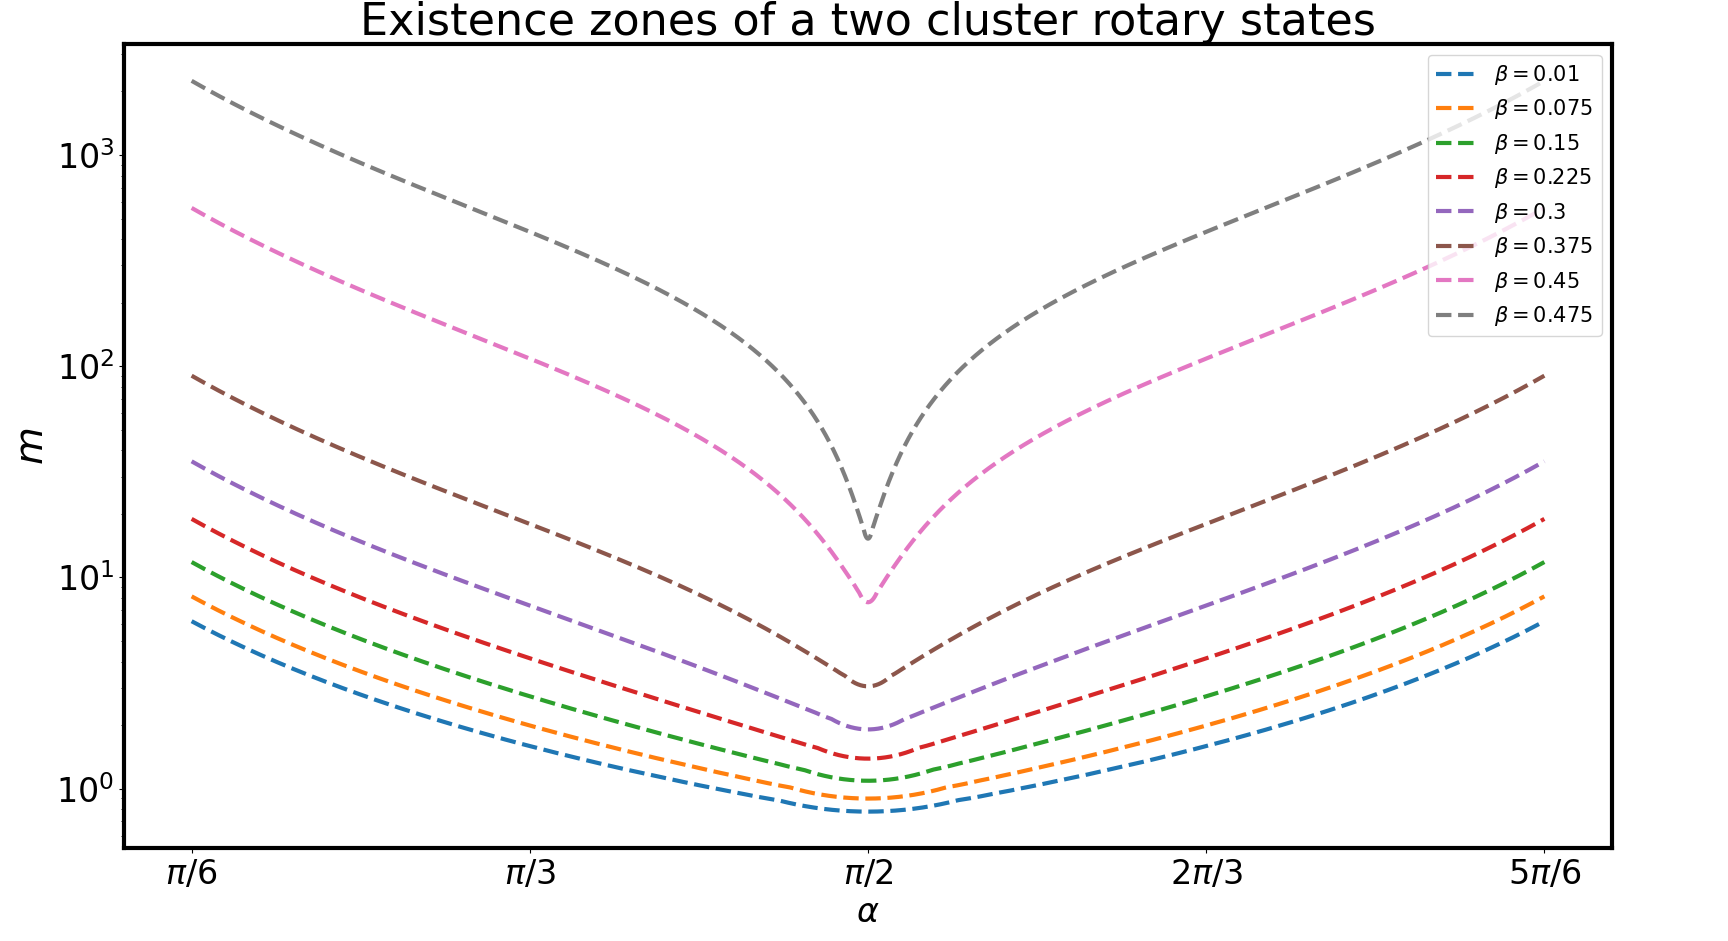
\includegraphics[width=1\columnwidth]{pictures/ex.png}
		\end{center}
		\caption{Границы зон устойчивости двухкластерного вращательного режима с вращающейся расстройкой фаз в зависимости от параметра $\beta$.}
		\label{ex-zones}
	\end{figure}

	На рисунке \ref{ex-zones} изображены границы зон устойчивости двухкластерного вращательного режима
	с вращающейся расстройкой фаз в зависимости от параметра $\beta$.
	Можно заметить, что при фиксированном $N$ зона существования двухкластерного режима при размере малого кластера равного $K_1$ полностью включена в 
	зону существования двухкластерного режима при размере малого кластера равного $K_2$ при $K_1 > K_2$. Наблюдается мультистабильность вращательных режимов.


	На рисунке \ref{schema} изображены двухкластерные вращательные режимы в зависимости от параметра $N$.
	Каждая ячейка представляет собой определенный двухкластерный режим,
	характеризующийся параметром $\beta$, который записан в виде несократимой дроби в центре ячейки. Ячейки с одинаковым цветом, кроме серого, представляют собой
	один и тот же двухкластерный вращательный режим. Несложно заметить, что при фиксированном $N = N^*$,
	двухкластерный вращательный режим, соответствующий $\beta^* = A/B$, где $A/B$ - несократимая дробь, 
	будет повторяться для всех $N = N^* + k\cdot B$. 

	\begin{figure}[h!]
		\begin{center}
			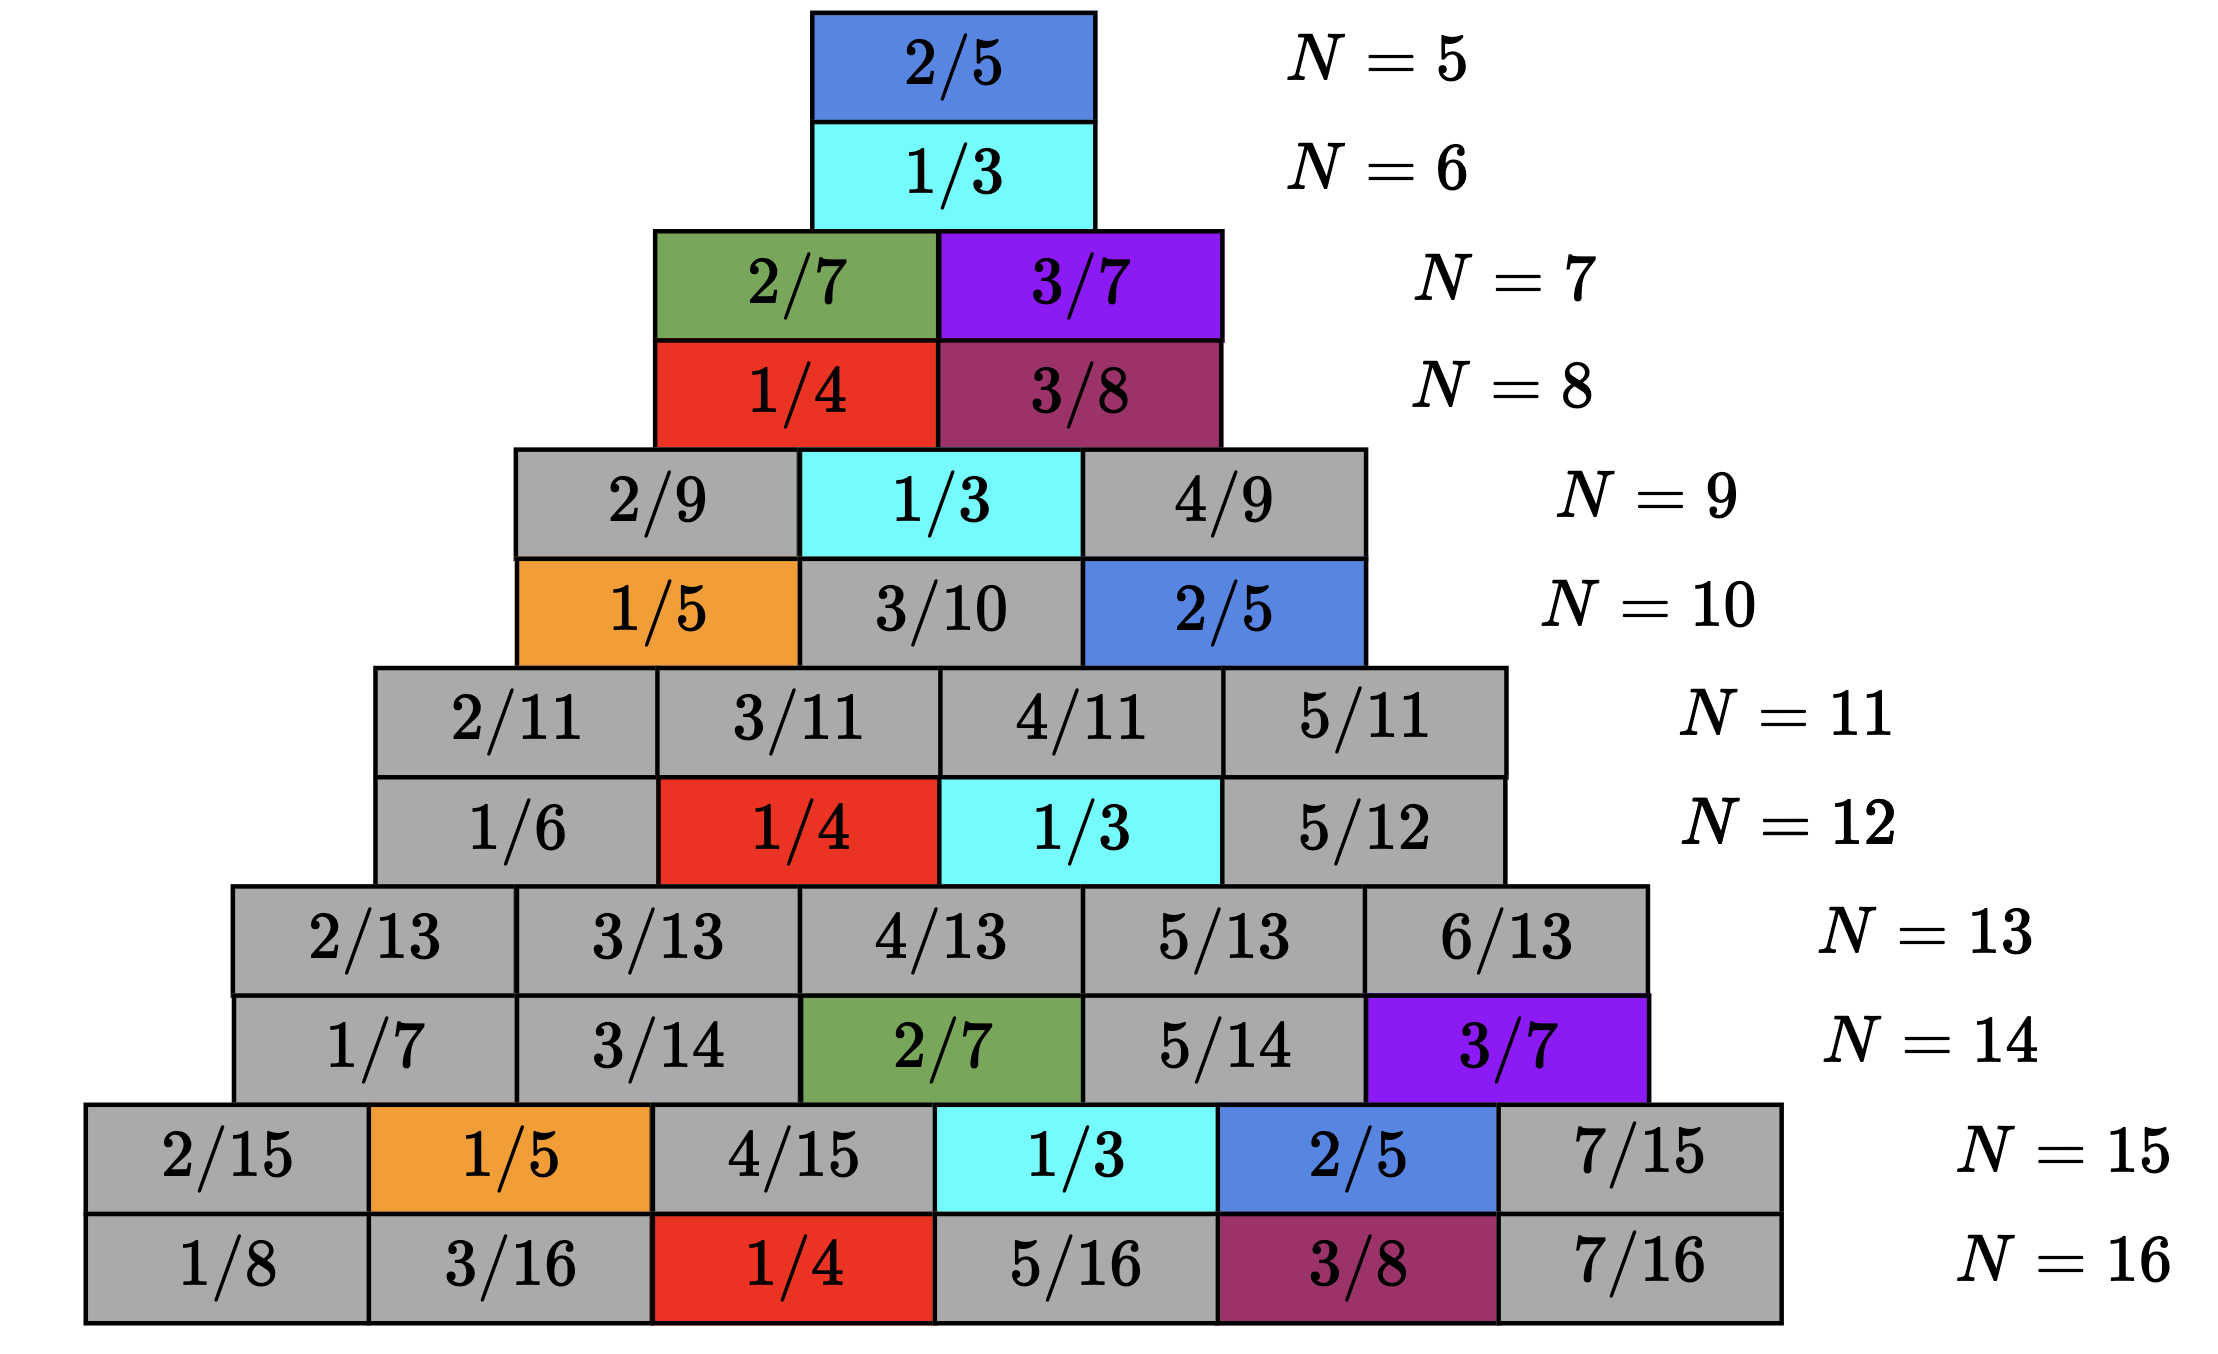
\includegraphics[width=1\columnwidth]{pictures/schema.png}
		\end{center}
		\caption{Двухкластерные вращательные режимы в зависимости от параметра $N$. Каждая ячейка представляет собой определенный двухкластерный режим,
		характеризующийся параметром $\beta$, который записан в виде несократимой дроби в центре ячейки. Ячейки с одинаковым цветом, кроме серого, представляют собой
		один и тот же двухкластерный вращательный режим.}
		\label{schema}
	\end{figure}

\end{chapter}
	\begin{chapter}{Устойчивость двухкластерных вращательных режимов}
	\section{Устойчивость двухкластерных вращательных движений с постоянной расстройкой фаз}
	
	Перепишем \ref{pre-pend} в виде системы:
	
	\begin{equation} \label{system}
		\begin{cases}
			\dot{x} = y, \\
			\dot{y} = \frac{1}{m} \left[ (1 - 2\beta)\sin{\alpha}(1 - \cos{x}) - \sin{x}\cos{\alpha} - y \right]
		\end{cases}
	\end{equation}
	
	Выполним линеаризацию системы \ref{system}:
	
	\begin{equation} \label{system-linear}
		\begin{pmatrix}
			\dot{\hat{x}} \\
			\dot{\hat{y}}
		\end{pmatrix}
		=
		\begin{pmatrix}
			0 & 1 \\
			\frac{1}{m}\left[ (1 - 2\beta)\sin{\alpha}\sin{x_p} - \cos{\alpha}\cos{x_p} \right] & -\frac{1}{m}
		\end{pmatrix}
		\begin{pmatrix}
			\hat{x} \\
			\hat{y}
		\end{pmatrix}
	\end{equation}
	Где $x_p$ - стационарные состояния системы \ref{pre-pend}. Характеристический многочлен системы \ref{system-linear}:
	
	\begin{equation} \label{hp}
		\lambda^2 + \frac{1}{m}\lambda - \frac{1}{m}\left[ (1 - 2\beta)\sin{\alpha}\sin{x_p} - \cos{\alpha}\cos{x_p} \right] = 0
	\end{equation}
	
	Из \ref{hp} можно заметить, что устойчивость стационарного состояния $x_p$ определяется соотношением:
	
	\begin{equation} \label{hp-stability}
		\cos{\alpha}\cos{x_p} - (1 - 2\beta)\sin{\alpha}\sin{x_p} > 0
	\end{equation}
	
	Несложно заметить, что стационарные состояния в уравнении \ref{pre-pend} определяются выражением:
	$$
	\sin{(x_p + \varphi)} = \frac{(1 - 2\beta) \sin{\alpha}}{\sqrt{\cos{\alpha}^2 + (1 - 2\beta)^2\sin{\alpha}^2}},
	$$
	Откуда:
	\begin{equation} \label{x1}
		x_{p_1} = \begin{cases}
			0, \alpha \in [-\pi/2, \pi/2) \\
			2\arcsin{\frac{(1 - 2\beta) \sin{\alpha}}{\sqrt{\cos{\alpha}^2 + (1 - 2\beta)^2\sin{\alpha}^2}}} - \pi , \alpha \in [\pi/2, 3\pi/2)
		\end{cases}
	\end{equation}
	
	\begin{equation} \label{x2}
	x_{p_2} = \begin{cases}
		\pi - 2\arcsin{\frac{(1 - 2\beta) \sin{\alpha}}{\sqrt{\cos{\alpha}^2 + (1 - 2\beta)^2\sin{\alpha}^2}}}, \alpha \in [-\pi/2, \pi/2) \\
		0, \alpha \in [\pi/2, 3\pi/2)
		\end{cases}
	\end{equation}
	
	Подставляя \ref{x1}, \ref{x2} в \ref{hp-stability}
	получаем, что $x_{p_1}$ - устойчива, $x_{p_2}$ - неустойчива.

	\begin{figure}[h!]\center		
		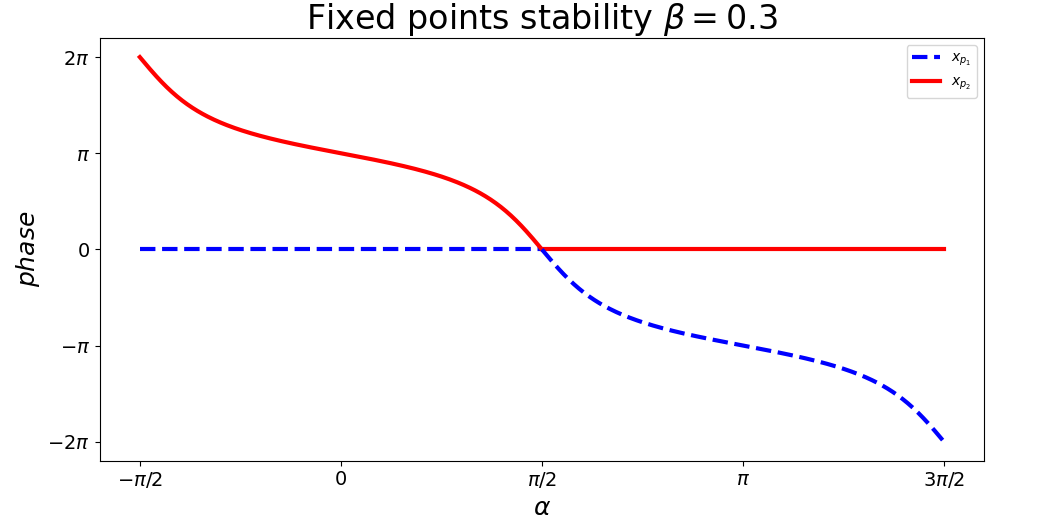
\includegraphics[width=1\columnwidth]{pictures/fixed-points.png} 
		\caption{\textbf{Устойчивость стационарных состояний.}
		Синяя пунктирная линия - устойчивое состояние $x_{p_1}$,
		Красная сплошная линия - неустойчивое состояние $x_{p_2}$.
		$\beta = 0.3$}
		\label{fp-2}
	\end{figure}

	\begin{figure}[h!]
		\begin{center}
			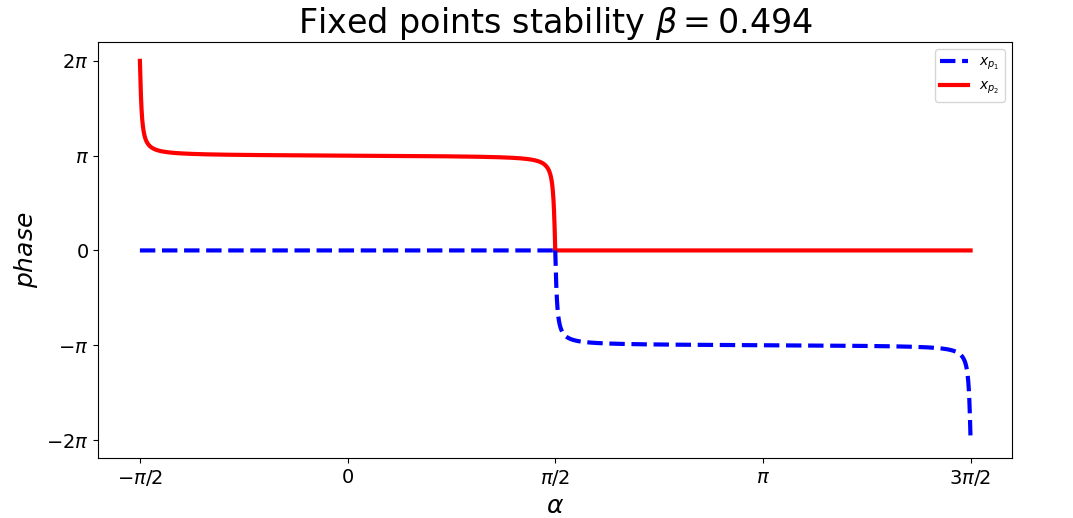
\includegraphics[width=1\columnwidth]{pictures/fixed-points-3.png}
		\end{center}
		\caption{\textbf{Устойчивость стационарных состояний.}
		Синяя пунктирная линия - устойчивое состояние $x_{p_1}$,
		Красная сплошная линия - неустойчивое состояние $x_{p_2}$.
		$\beta = 0.494$}
		\label{fp-3}
	\end{figure}

	На рисунке \ref{fp-2} изображены стационарные состояния уравнения \ref{pre-pend} при параметре $\beta = 0.3$.
	Синей пунктирной линией отмечены устойчивые стационарные состояния,
	красной сплошной - неустойчивые. При $\alpha \in [-\pi/2, \pi/2)$ $x_{p_1} = 0$ и является устойчивой, что соответствует
	устойчивому синфазному вращательному режиму в исходной системе. Это естественно, ведь при $\alpha \in [-\pi/2, \pi/2)$ связь является
	притягивающей. Заметим, что при $\beta$ стремящейся к 0.5 стационарные состояния с расстройкой фаз неравной нулю стремятся
	к $\pi k$, $k \in \mathbb{Z}$ (см.рис. \ref{fp-3}).
	Стоит отметить, что в полной системе \ref{main-sistem} двухкластерное вращательное движение с постоянной расстройкой фаз $X = x_{p_1}$
	может терять свою устойчивость. Данный эффект будет продемонстрирован в следующем разделе, посвященном устойчивости.
	Таким образом нас будет интересовать только устойчивость двухкластерных состояний с периодической расстройкой фаз.
	
	\section{Устойчивость двухкластерных вращательных движений с периодической расстройкой фаз}

	Выполним линеаризацию относительно произвольного вращательного движения $\psi_i$ с помощью замены $\varphi_i = \psi_i + \delta_i$, где вариации $\delta_i$ малы:
	\begin{equation} \label{pretubr}
		m\ddot{\delta}_i + \dot{\delta}_i = \frac{1}{N} \sum_{j = 1}^N \cos{(\psi_j - \psi_i - \alpha)} \cdot (\delta_j - \delta_i), \ i = \overline{1, N}
	\end{equation}
	Для случая двухкластерного режима \ref{two-cluster} система \ref{pretubr} запишется в виде:
	
	\begin{equation}
		\begin{cases}
			m\ddot{\delta}_i + \dot{\delta}_i = \frac{1}{N} \left( \cos{\alpha} \sum_{j = 1}^K (\delta_j - \delta_i) + \cos{(X + \alpha)} \sum_{j = K + 1}^N (\delta_j - \delta_i) \right), \ i = \overline{1,K}, \\
			m\ddot{\delta}_i + \dot{\delta}_i = \frac{1}{N} \left( \cos{(X - \alpha)} \sum_{j = 1}^K (\delta_j - \delta_i) +  \cos{\alpha} \sum_{j = K + 1}^N (\delta_j - \delta_i)  \right), \ i = \overline{K + 1,N},
		\end{cases}		
	\end{equation}
	
	Выполняя замену:
	\begin{align*}
		\eta_1 = \frac{1}{K} \sum_{i = 1}^K \delta_i - \frac{1}{N - K} \sum_{i = K + 1}^N \delta_i, \\
		\eta_2 = \frac{1}{K} \sum_{i = 1}^K \delta_i + \frac{1}{N - K} \sum_{i = K + 1}^N \delta_i, \\
		\xi_n = \delta_{n+1} - \delta_n, \ 1 \leq  n \leq K - 1, \\
		\zeta_n = \delta_{n+1} - \delta_n, \ K + 1 \leq n \leq N - 1.
	\end{align*}
		
	Приходим к системе уравнений:
	
	\begin{equation} \label{split-linear-pert-sys-n12}
		\begin{cases}
			m\ddot{\eta}_1 + \dot{\eta}_1 + \left( \beta \cos{(X - \alpha)} + (1 - \beta) \cos{(X + \alpha)} \right) \eta_1 = 0, \\
			m\ddot{\eta}_2 + \dot{\eta}_2 + \left( (1 - \beta) \cos{(X + \alpha)} - \beta \cos{(X - \alpha)} \right) \eta_1 = 0,
		\end{cases}
	\end{equation}
	
	
	\begin{equation} \label{split-linear-pert-sys-ksi-eta}
		\begin{cases}
			m\ddot{\xi}_n + \dot{\xi}_n + \left( (1 - \beta) \cos{(X + \alpha)} + \beta \cos{\alpha} \right) \xi_n = 0, \\
			m\ddot{\zeta}_n + \dot{\zeta}_n + \left( (1 - \beta) \cos{\alpha} + \beta \cos{(X - \alpha)} \right) \zeta_n = 0.
		\end{cases}
	\end{equation}
	
	Так как $X$ периодична, мы можем применить теорию Флоке
	и найти мультипликаторы, определяющие асимптотическое поведение решений системы.
	
	Проанализируем систему \ref{split-linear-pert-sys-n12} (переменные $\eta_1$, $\eta_2$).
	Из \ref{pre-pend} следует, что одним из
	решений первого уравнения является $\dot{X}$.
	Так как $X$ периодична, то один из мультипликаторов равен 1.
	Согласно формуле Лиувилля-Остроградского, второй мультипликатор первого уравнения равен $\exp{(-\frac{T_x}{m})}$.
	Кроме того, полная система имеет решение $\eta_1 = 0$, $\eta_2 = const$,
	откуда следует, что еще один мультипликатор равен единице.
	Вновь применяя формулу Лиувилля-Остроградского, но
	уже ко всей системе, находим четвертый мультипликатор,
	равный $\exp{(-\frac{T_x}{m})}$. 
	Итак, рассматриваемый режим всегда внутренне устойчив.

	
	Проанализируем систему \ref{split-linear-pert-sys-ksi-eta} (переменные $\xi$, $\zeta$).
	Переменная $\xi$ соответствует малому кластеру, переменная $\zeta$ соответствует большому кластеру. 
	Они не связанны между собой.
	Благодаря такому разделению переменных, мы можем проследить как меняется устойчивость
	двухкластерного режима с периодической расстройкой фаз для каждого кластера. В зависимости от $X$ устойчивость
	может пропасть или появится только у одного или сразу у двух кластеров, благодаря чему мы можем
	понять каким образом двухкластерный режим будет разрушаться в случае потери устойчивости.
	
	С помощью уравнений \ref{split-linear-pert-sys-ksi-eta} определим устойчивость стационарного
	двухкластерного вращательного режима, соответствующего состоянию $x_{p_1}$.
	Уравнения запишутся в виде:
	
	\begin{equation}
		x_{p_1} = 0, \ \alpha \in [-\pi/ 2, \pi/2]: 
		\begin{cases}
			m\ddot{\xi}_n + \dot{\xi}_n + \cos{\alpha}\xi_n = 0, \\
			m\ddot{\zeta}_n + \dot{\zeta}_n + \cos{\alpha}\zeta_n = 0.
		\end{cases}
	\end{equation}
	
	\begin{equation}
		\begin{split}
			x_{p_1} = 2\arcsin{\frac{(1 - 2\beta) \sin{\alpha}}{\sqrt{\cos{\alpha}^2 + (1 - 2\beta)^2\sin{\alpha}^2}}} - \pi , \alpha \in [\pi/2, 3\pi/2): \\ 
			:\begin{cases}
				m\ddot{\xi}_n + \dot{\xi}_n + A(\alpha, \beta) \xi_n = 0, \\
				m\ddot{\zeta}_n + \dot{\zeta}_n -A(\alpha, \beta) \zeta_n = 0.
			\end{cases}
		\end{split}
	\end{equation}
	Где $A$ - некоторый коэффициент. Заметим, что при $\alpha \in [-\pi/ 2, \pi/2)$, $x_{p_1}$ - устойчива в исходной системе,
	при $\alpha \in [\pi/2, 3\pi/2)$, $x_{p_1}$ - неустойчива в исходной системе.

	Получается, что в исходной системе двухкластерный вращательный режим с постоянной расстройкой фаз всегда является неустойчивым.
	Таким образом дальнейший анализ устойчивости мы будем проводить только для двухкластерных вращательных движений с периодической
	расстройкой фаз.


	В результате численного моделирования были получены карты устойчивости двухкластерных вращательных
	режимов с периодической расстройкой фаз в области параметров $\alpha$, $m$. Из рисунка \ref{map-083} видно, что устойчивость двухкластерного режима разрушается из - за потери устойчивости у одного из кластеров:
	как большого при больших значениях параметра $\alpha$, так и малого при меньших значениях параметра $\alpha$.
	Можно заметить, что внутри зоны устойчивости большого кластера появляется зона параметрической неустойчивости при $\beta \approx 0.25$ (см. рис. \ref{map-025}), которая
	разрастается с увеличением параметра $\beta$ (см. рис. \ref{map-0-292}, \ref{map-0-33}). При $\beta \approx 0.375$ (см. рис. \ref{map-0375}) зона устойчивости большого кластера
	распадается на две несвязных компоненты. При увеличении параметра $\beta$ область устойчивости двухкластерного вращательного движения смещается в область отталкивающей связи.
	На рисунке \ref{st-c-1} изображена пространственно-временная диаграмма для $N = 24$ элементов из области параметров, когда
	двухкластерный вращательный режим является устойчивым. Моделирование системы выполнялось с начальными условиями 
	близкими к реализации двухкластерного вращательного режима. Из рисунка \ref{st-c-1} видно, что даже при наличии возмущений,
	спустя некоторое время в системе устанавливается двухкластерный вращательный режим с периодической расстройкой фаз, что согласуется с
	картой устойчивости \ref{map-0125}. Результаты других пространственно-временных диаграмм также согласуются с картами устойчивости двухкластерного вращательного режима.
	Таким образом корректность карт устойчивости, которые были получены с помощью редуцированной системы, подтверждены прямым численным моделированием в полной системе (см. рис. \ref{st-c-1}, \ref{st-c-2}, \ref{st-c-3}, \ref{st-c-4}).
	На рисунке \ref{su-map} изображена карта устойчивости двухкластерных вращательных состояний с
	периодической расстройкой фаз в зависимости от размеров малого кластера. Более темный цвет
	характеризуется большей мультистабильностью двухкластерных вращательных движений.
	Чем больше размер малого кластера, тем меньше соответствующая
	зона устойчивости. Также при увеличении размеров малого кластера увеличивается максимально возможное значение параметра
	$\alpha$, при котором двухкластерное вращательное движение сохраняет свою устойчивость.
	Наблюдается небольшая область устойчивости двухкластерного вращательного движения при параметрах $\alpha > \pi/2$, что соответствует
	реализации отталкивающей связи. При увеличении размеров малого кластера эта область также увеличивается в размерах.

	\begin{figure}[h!]\center
		
		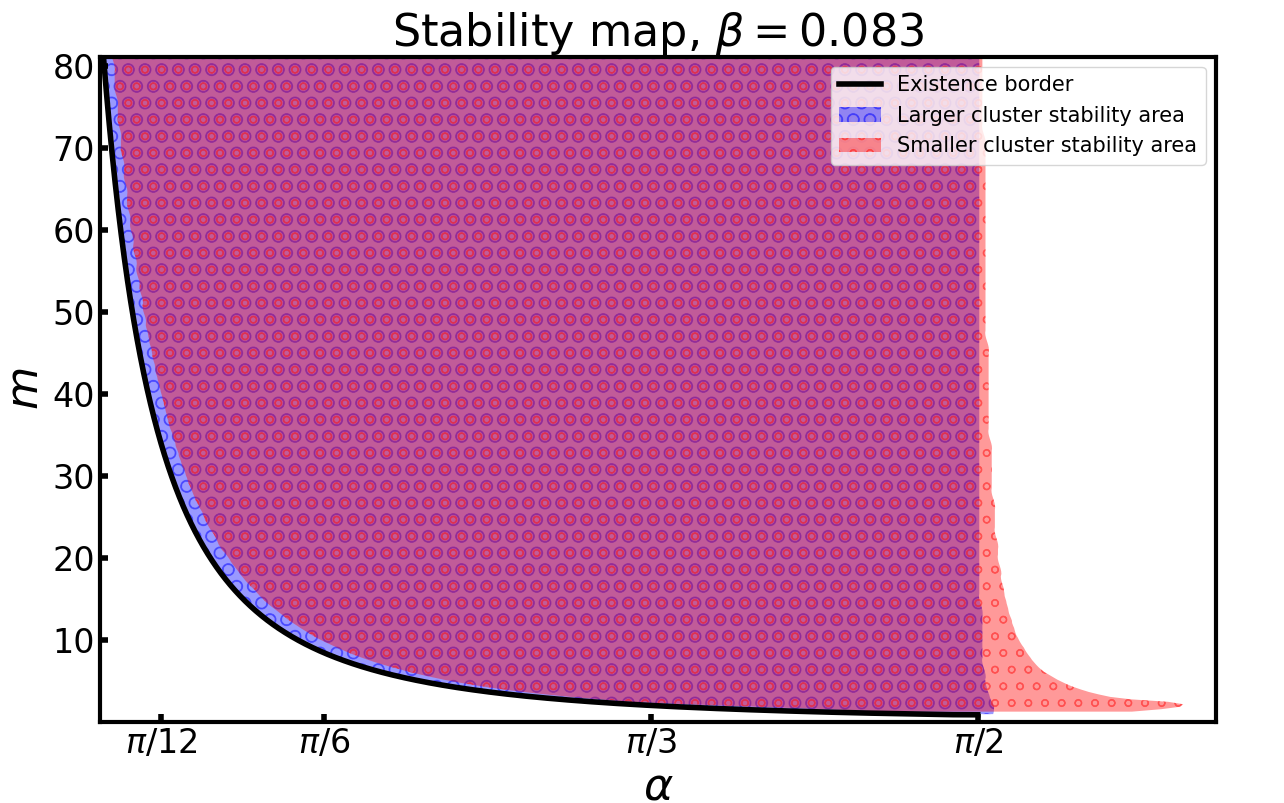
\includegraphics[width=1\columnwidth]{pictures/map-0-083.png}
		\caption{\textbf{Карта устойчивости двухкластерных вращательных состояний с периодической расстройкой фаз.}
		Область с малыми маркерами соответствует устойчивости малого кластера.
		Область с большими маркерами соответствует устойчивости большого кластера.
		На пересечении этих областей двухкластерный вращательный режим с периодической расстройкой фаз является устойчивым}
		\label{map-083}
	\end{figure}


	\begin{figure}[h!]\center
		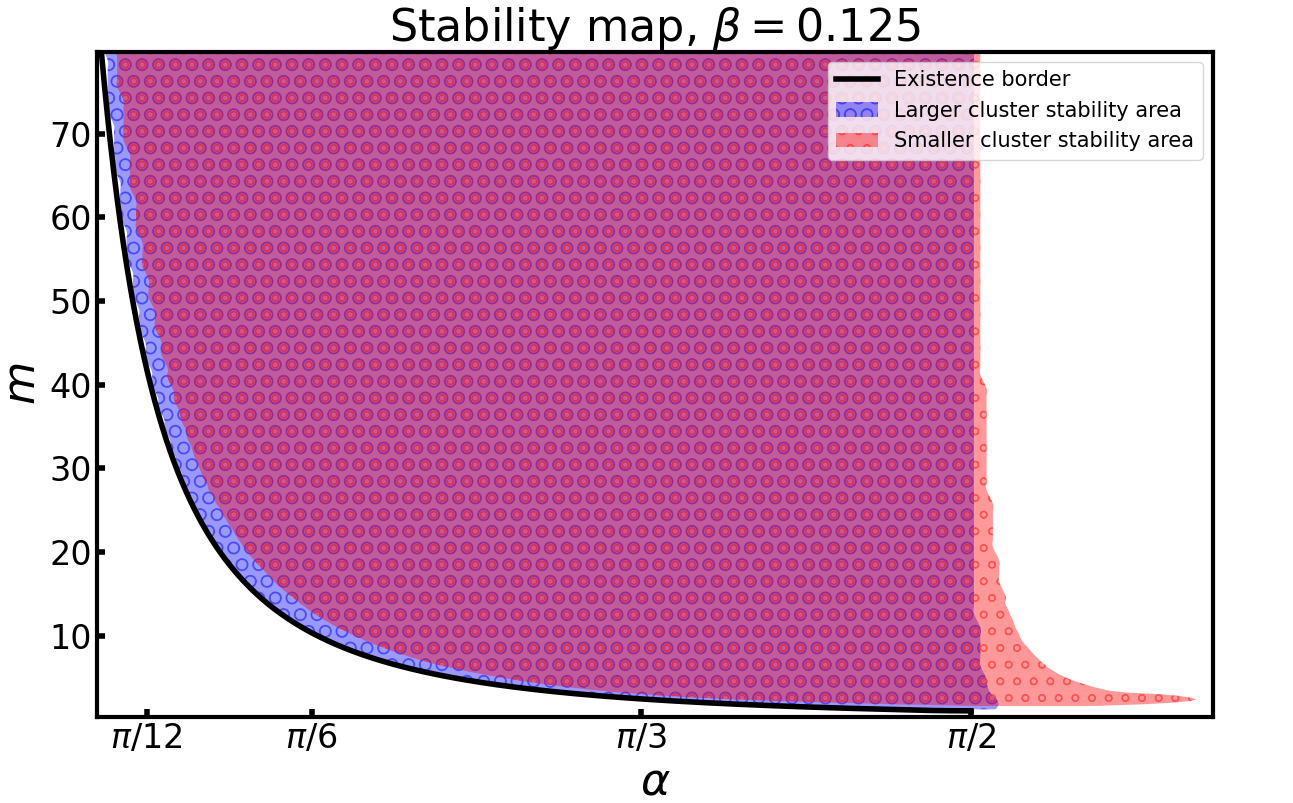
\includegraphics[width=1\columnwidth]{pictures/map-0-0125.png}
		\caption{\textbf{Карта устойчивости двухкластерных вращательных состояний с периодической расстройкой фаз.}
		Область с малыми маркерами соответствует устойчивости малого кластера.
		Область с большими маркерами соответствует устойчивости большого кластера.
		На пересечении этих областей двухкластерный вращательный режим с периодической расстройкой фаз является устойчивым}
		\label{map-0125}
	\end{figure}

	
	\begin{figure}[h!]\center
		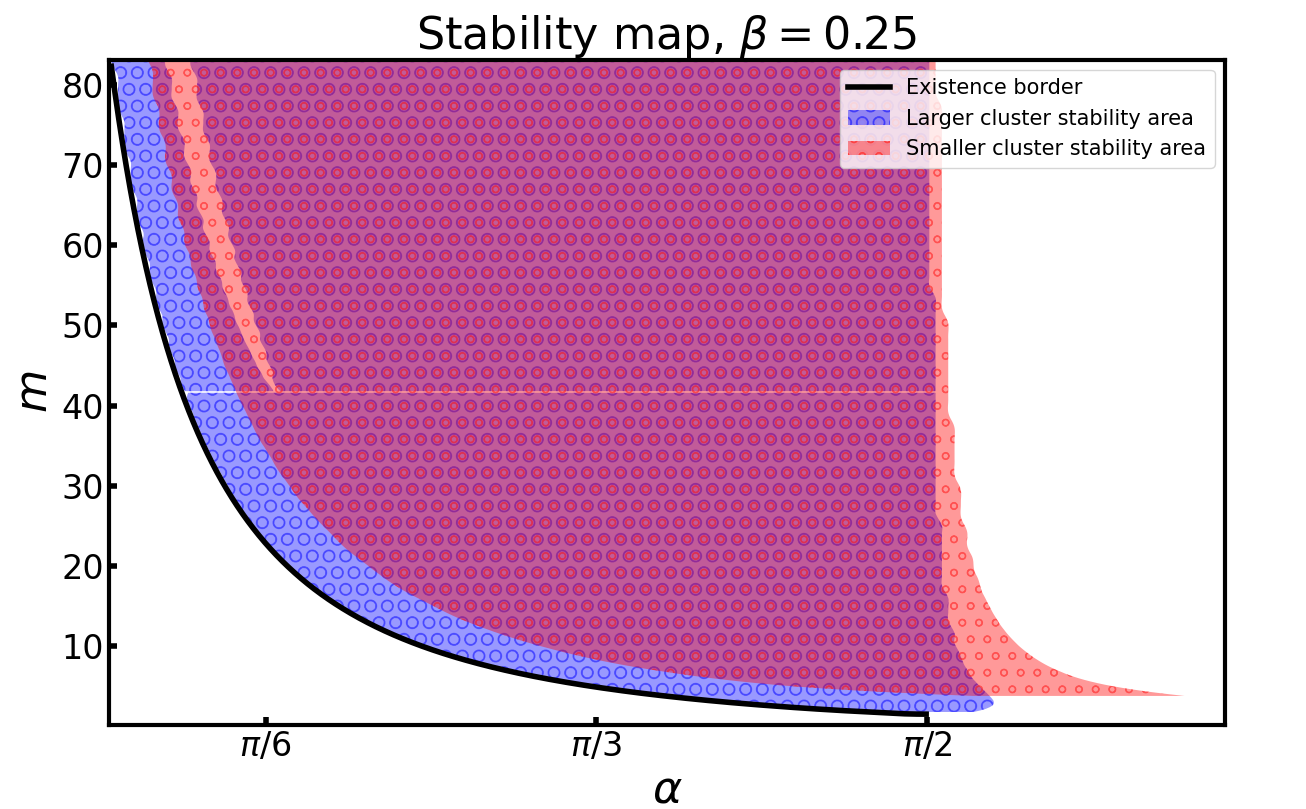
\includegraphics[width=1\columnwidth]{pictures/map-0-25.png}
		\caption{\textbf{Карта устойчивости двухкластерных вращательных состояний с периодической расстройкой фаз.}
		Область с малыми маркерами соответствует устойчивости малого кластера.
		Область с большими маркерами соответствует устойчивости большого кластера.
		На пересечении этих областей двухкластерный вращательный режим с периодической расстройкой фаз является устойчивым}
		\label{map-025}
	\end{figure}


	\begin{figure}[h!]\center
		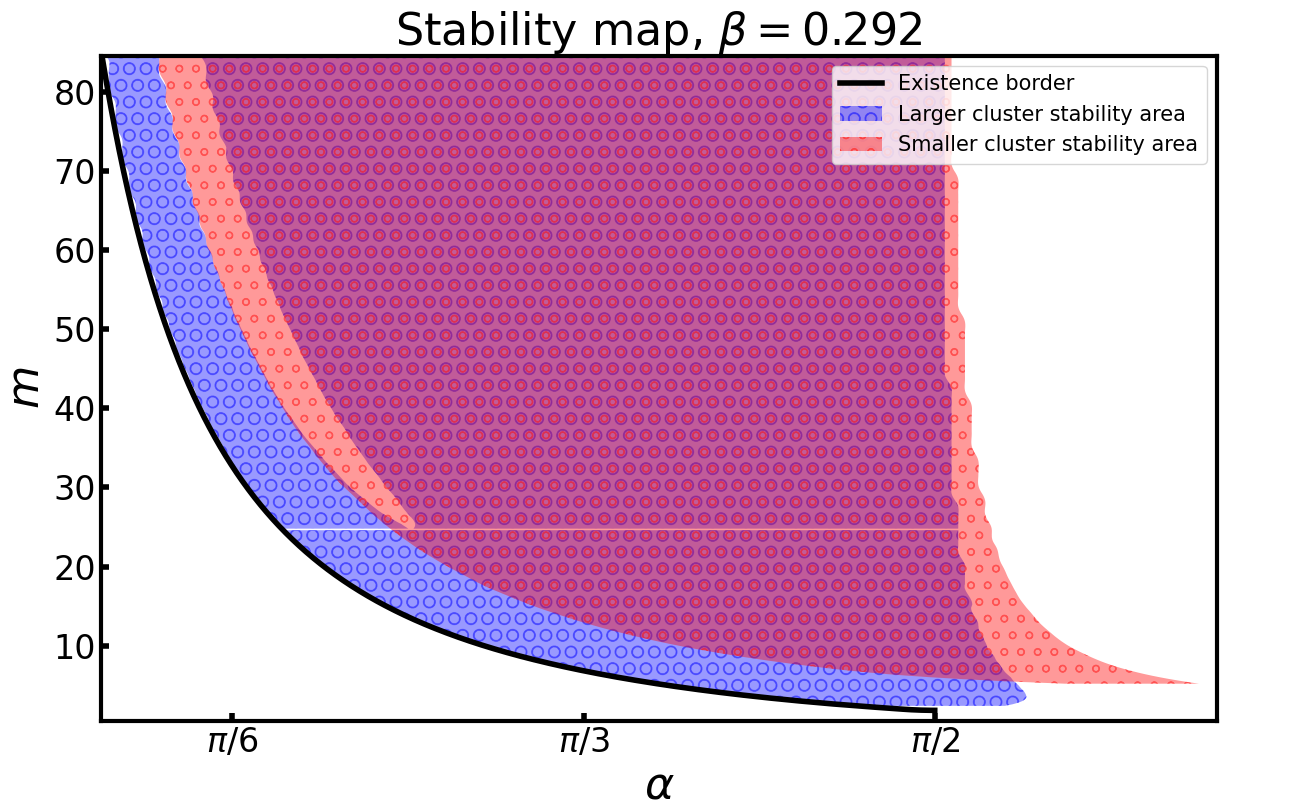
\includegraphics[width=1\columnwidth]{pictures/map-0-292.png}
		\caption{\textbf{Карта устойчивости двухкластерных вращательных состояний с периодической расстройкой фаз.}
		Область с малыми маркерами соответствует устойчивости малого кластера.
		Область с большими маркерами соответствует устойчивости большого кластера.
		На пересечении этих областей двухкластерный вращательный режим с периодической расстройкой фаз является устойчивым}
		\label{map-0-292}
	\end{figure}

	\begin{figure}[h!]\center
		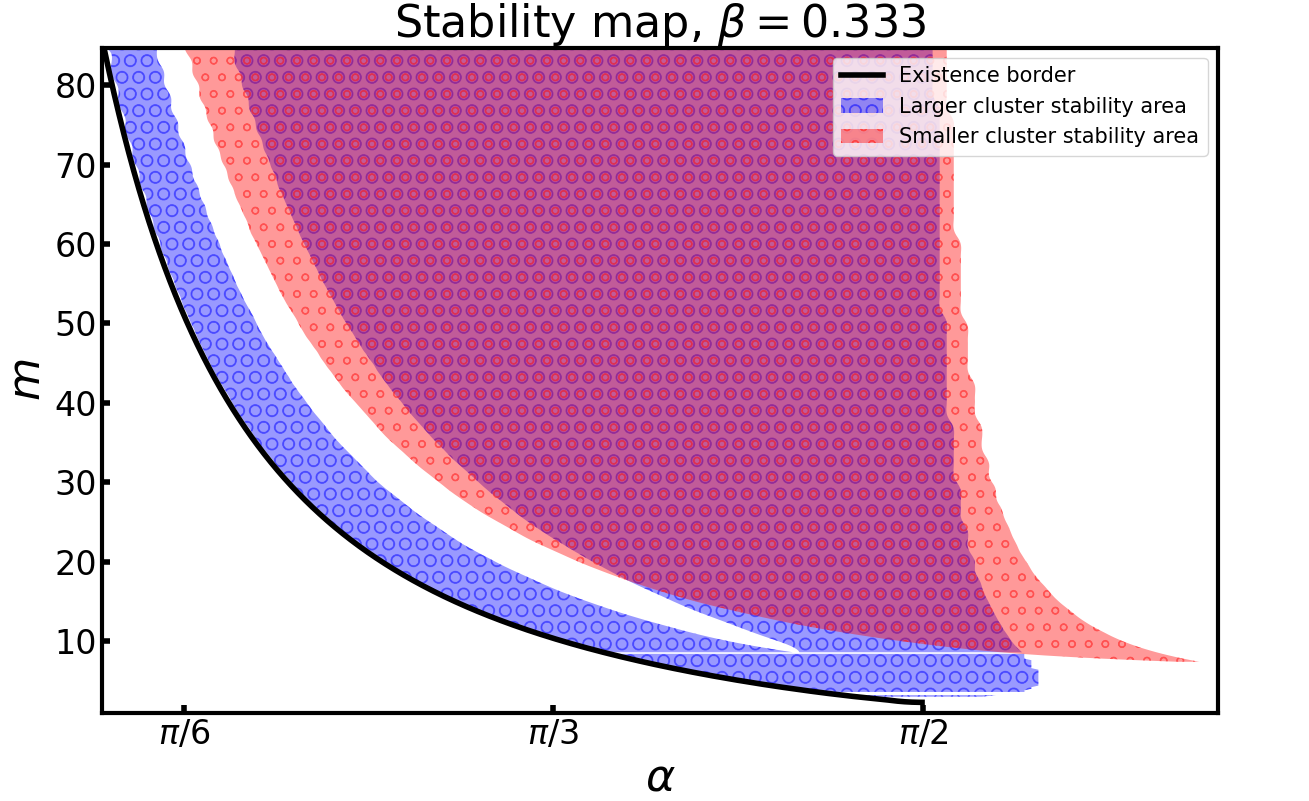
\includegraphics[width=1\columnwidth]{pictures/map-0-33.png}
		\caption{\textbf{Карта устойчивости двухкластерных вращательных состояний с периодической расстройкой фаз.}
		Область с малыми маркерами соответствует устойчивости малого кластера.
		Область с большими маркерами соответствует устойчивости большого кластера.
		На пересечении этих областей двухкластерный вращательный режим с периодической расстройкой фаз является устойчивым}
		\label{map-0-33}
	\end{figure}


	\begin{figure}[h!]\center
		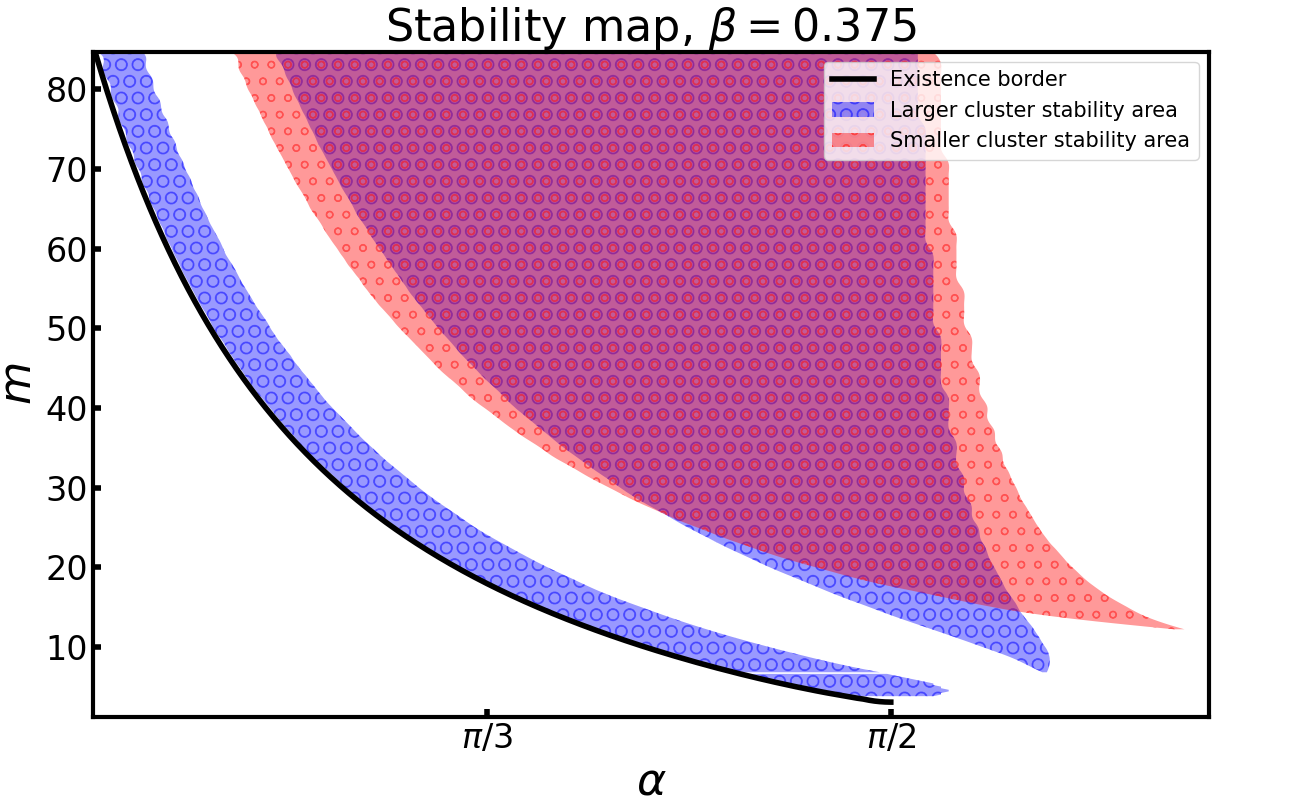
\includegraphics[width=1\columnwidth]{pictures/map-0-375.png}
		\caption{\textbf{Карта устойчивости двухкластерных вращательных состояний с периодической расстройкой фаз.}
		Область с малыми маркерами соответствует устойчивости малого кластера.
		Область с большими маркерами соответствует устойчивости большого кластера.
		На пересечении этих областей двухкластерный вращательный режим с периодической расстройкой фаз является устойчивым}
		\label{map-0375}
	\end{figure}

	\begin{figure}[h!]\center
		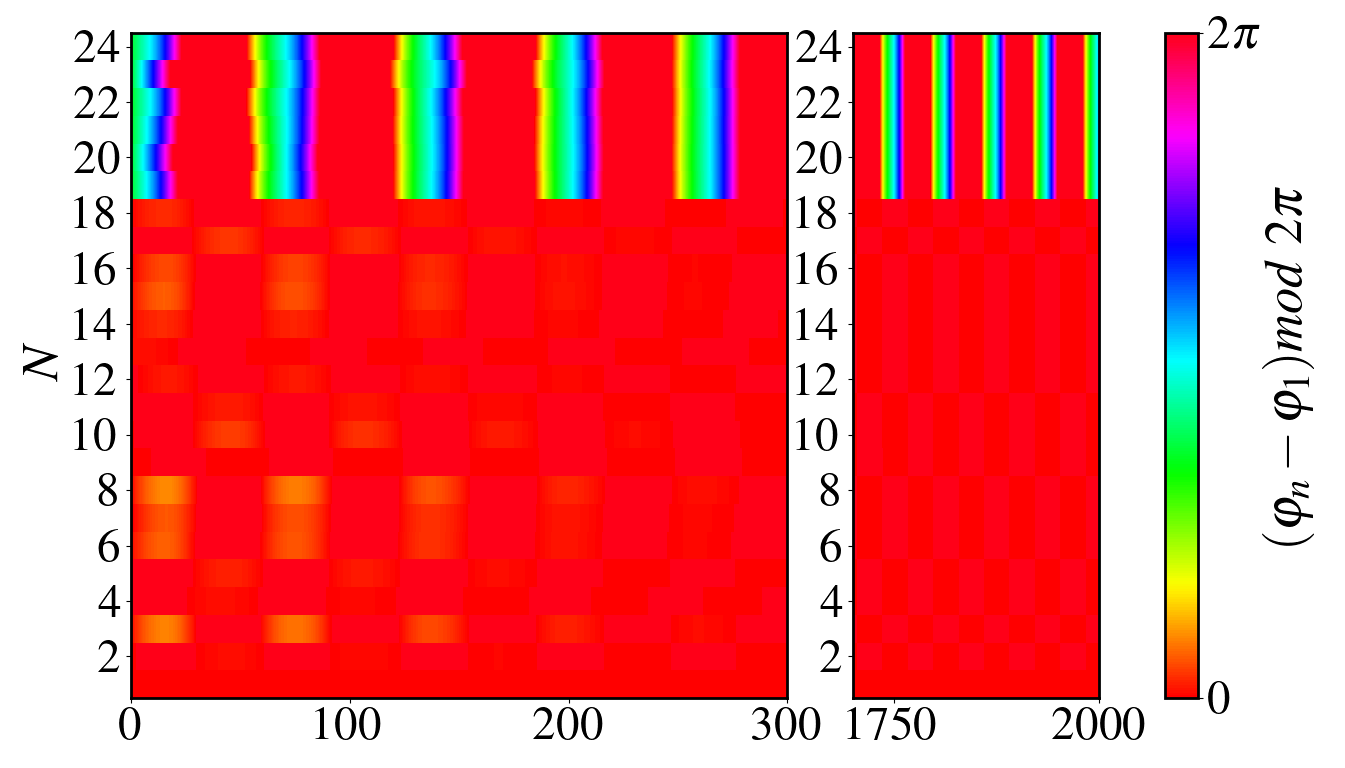
\includegraphics[width=1\columnwidth]{pictures/Figure_M_50_A_0.4586_O_1.png}
		\caption{\textbf{Пространственно-временная диаграмма.}
		Пространственно-временая диаграмма изображена для каждого элемента, относительно первого элемента.
		Цвет характеризует фазу элемента. Параметры: $N=24$, $m = 50$, $\omega = 1$, $\alpha = 0.4586$ (см. рис. \ref{map-025})}
		\label{st-c-1}
	\end{figure}

	\begin{figure}[h!]\center
		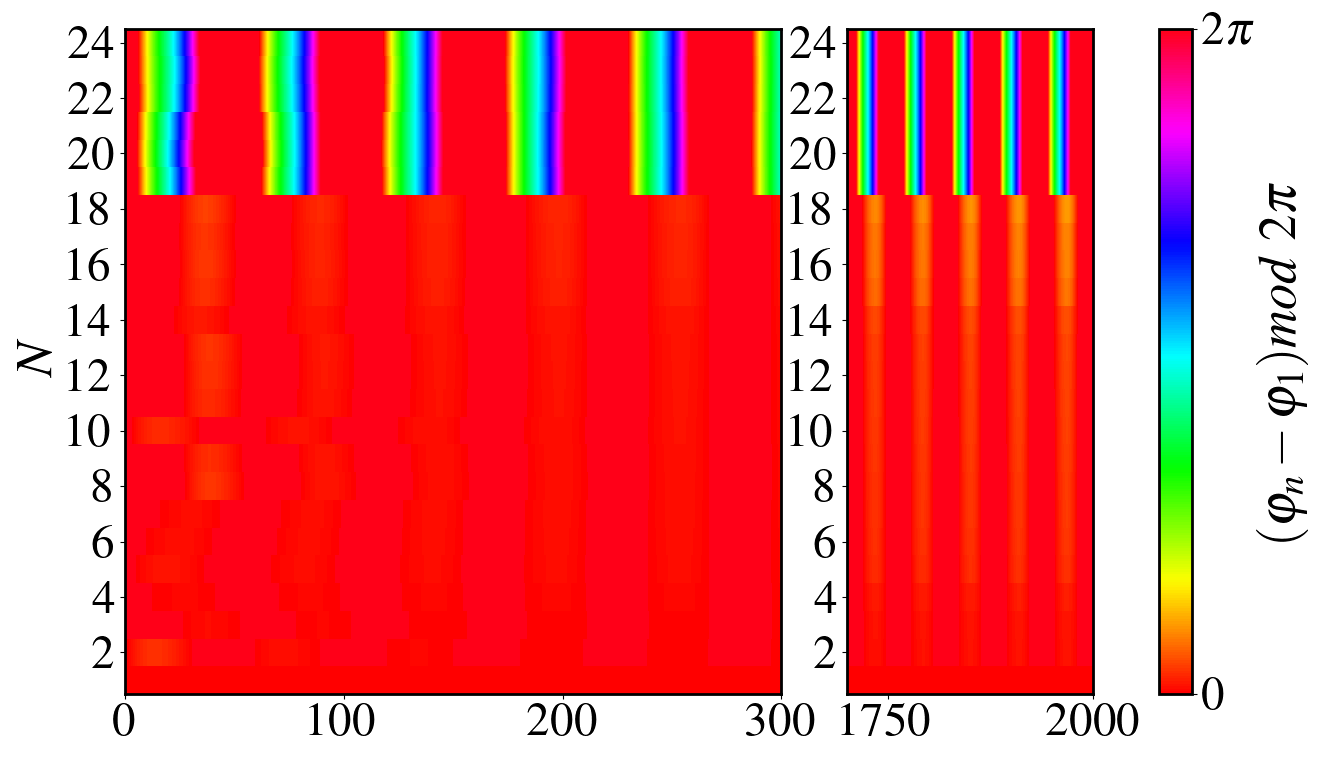
\includegraphics[width=1\columnwidth]{pictures/Figure_M_50_A_0.4946_O_1.png}
		\caption{\textbf{Пространственно-временная диаграмма.}
		Пространственно-временая диаграмма изображена для каждого элемента, относительно первого элемента.
		Цвет характеризует фазу элемента. Параметры: $N=24$, $m = 50$, $\omega = 1$, $\alpha = 0.4946$ (см. рис. \ref{map-025})}
		\label{st-c-2}
	\end{figure}

	\begin{figure}[h!]
		\begin{center}
			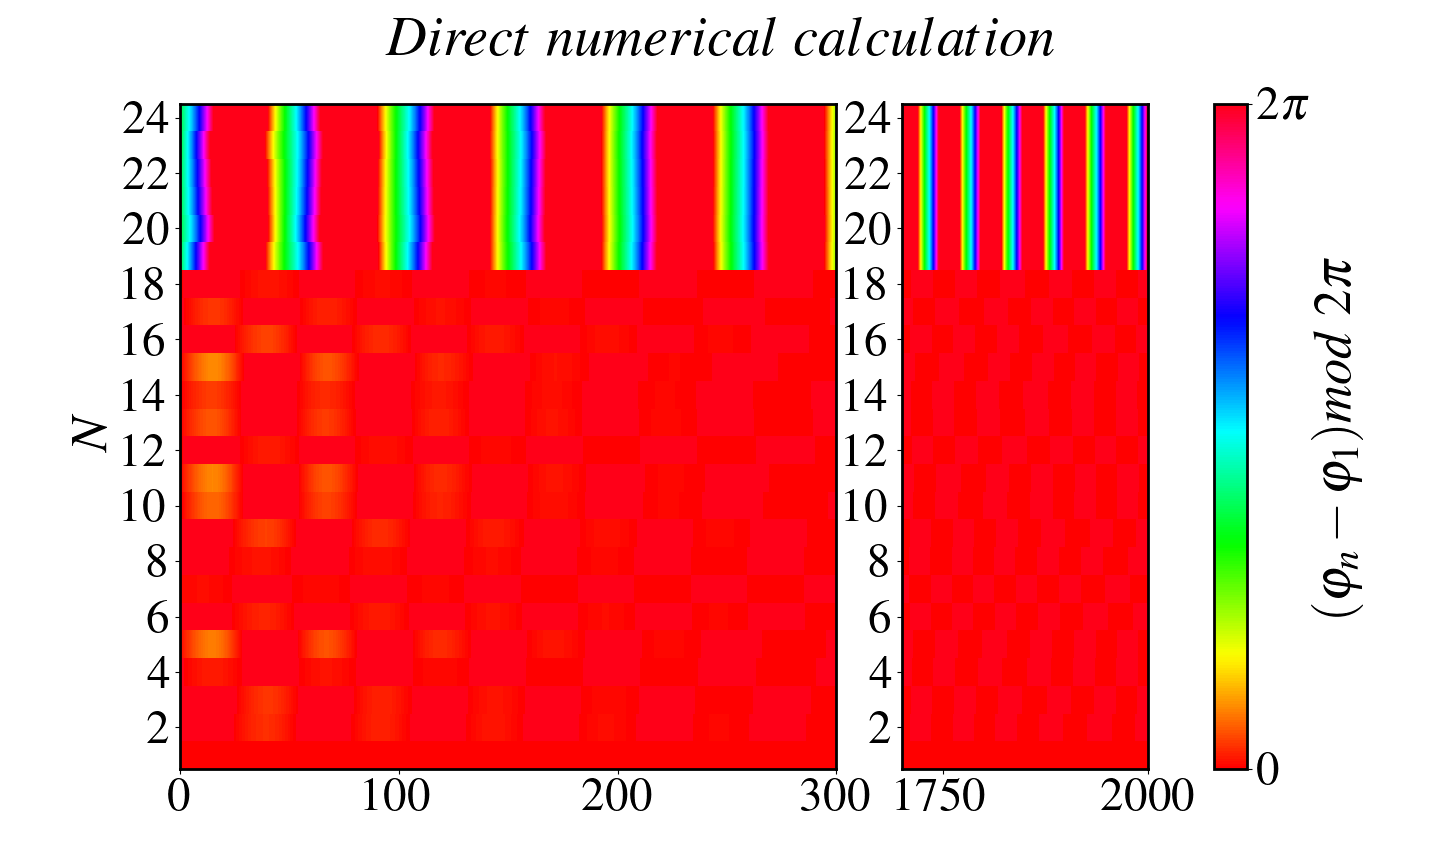
\includegraphics[width=1\columnwidth]{pictures/Figure_M_50_A_0.54_O_1.png}
		\end{center}
		\caption{\textbf{Пространственно-временная диаграмма.}
		Пространственно-временая диаграмма изображена для каждого элемента, относительно первого элемента.
		Цвет характеризует фазу элемента. Параметры: $N=24$, $m = 50$, $\omega = 1$, $\alpha = 0.54$ (см. рис. \ref{map-025})}
		\label{st-c-3}
	\end{figure}

	\begin{figure}[h!]
		\begin{center}
			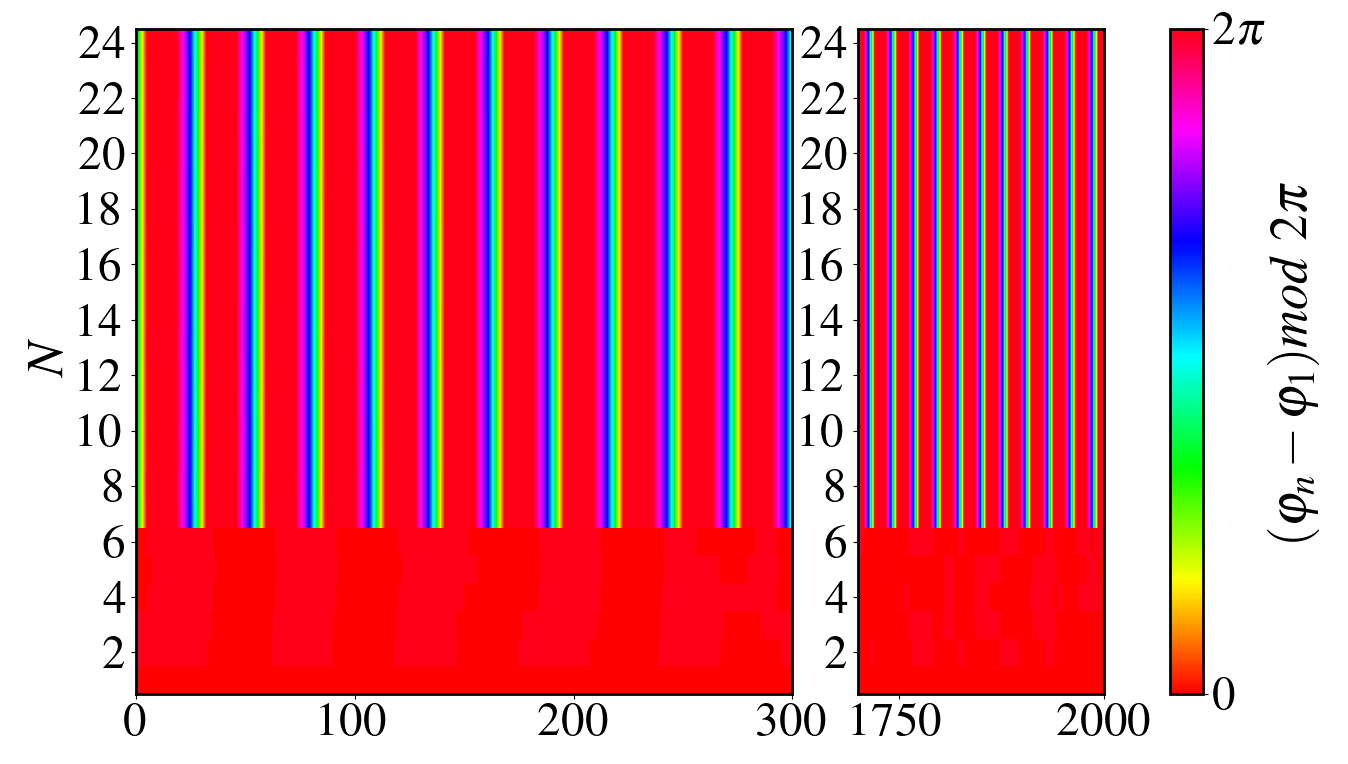
\includegraphics[width=1\columnwidth]{pictures/Figure_d.png}
		\end{center}
		\caption{\textbf{Пространственно-временная диаграмма.}
		Пространственно-временая диаграмма изображена для каждого элемента, относительно первого элемента.
		Цвет характеризует фазу элемента. Параметры: $N=24$, $m = 6.6$, $\omega = 1$, $\alpha = 1.6$ (см. рис. \ref{map-025})}
		\label{st-c-4}
	\end{figure}

	\begin{figure}[h!]
		\begin{center}
			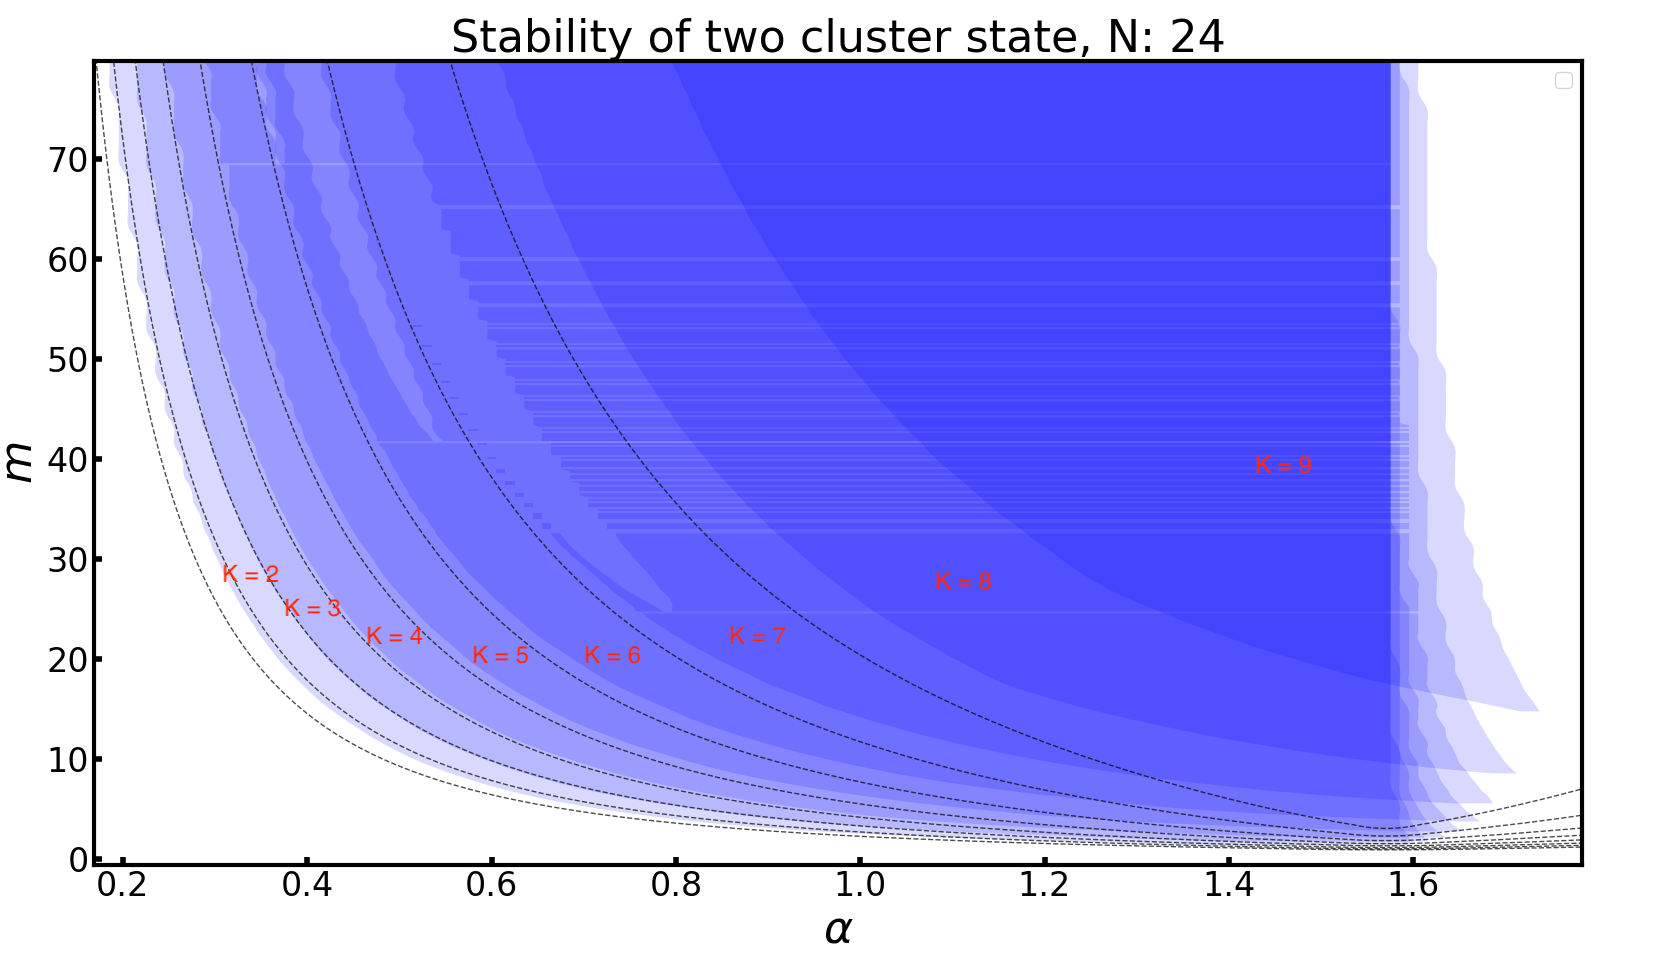
\includegraphics[width=1\columnwidth]{pictures/st-map.png}
		\end{center}
		\caption{\textbf{Карта устойчивости двухкластерных вращательных состояний с периодической расстройкой фаз в зависимости от размеров малого кластера.}
		Количество элементов $N = 24$. Внутри синей зоны двухкластерный режим является устойчивым. Черная пунктирная линия показывает
		границы существования двухкластерного вращательного режима. Текст, выделенный красным цветом, показывает количество элементов в малом
		кластере и располагается над соответствующей зоной устойчивости.}
		\label{su-map}
	\end{figure}

\end{chapter}
  \begin{chapter}{Программный комплекс}

	Программный комплекс, описываемый в этой главе, позволяет находить вращательные движения и
	определять их устойчивость в системах связанных фазовых элементов, которые описываются системой обыкновенных
	дифференциальных уравнений.

\section{Описание алгоритмов нахождения вращательных движений и определения их устойчивости}
	Для того, чтобы воспроизвести интересующее вращательное движение, необходимо иметь
	начальные условия и период вращательного движения. Для нахождения этих величин предлагается использовать
	алгоритмы для нахождения нулей некоторой многомерной функции, подробное устройство которой описано в \cite{Khorkin}.
	Для этого можно использовать метод Ньютона.
	Анализ устойчивости может быть произведен в рамках теории Флоке. Для этого необходимо найти
	собственные числа матрицы монодромии некоторой линейной системы с периодическими коэффициентами.
	Данная линейная система описывает динамику вариаций относительно найденного вращательного режима. Если все собственные числа матрицы монодромии находятся в пределах
	единичной окружности комплексной плоскости, рассматриваемый вращательный режим является линейно устойчивым.
	Стоит отметить тот факт, что для нахождения матрицы монодромии происходит интегрирование сразу двух систем одновременно:
	полной, в которой реализуется вращательное движение, а также линейной, из которой составляется матрица монодромии.  
\section{Описание структуры программного комплекса}
Программный комплекс написан на языке программирования python с использованием таких
библиотек как scipy \cite{scipy}, numpy \cite{numpy} и numba \cite{numba}.
Были реализованы три главных модуля: модуль интегрирования, модуль нахождения нулей многомерной функции, модуль, выполняющий расчет
матрицы монодромии.
Особый интерес представляет библиотека numba, которая реализует процедуру 
компиляции python кода в машинный код во время исполнения (jit compilation).
В частности, компиляция во время исполнения выполняется для функций, описывающих динамику системы.
Благодаря этому нахождение вращательных движений и определение их устойчивости реализованно эффективно.
В программном комплексе присутствует набор тестов \cite{testing}, проверяющих корректность работы главных алгоритмов.

\section{Модуль численного интегрирования}
Данный модуль позволяет произвести численное интегрирование систем обыкновенных
дифференциальных уравнений, тем самым решить задачу Коши:

$$
\dot{X} = F(X, t), \ X \in \mathbb{R}^n, \ t \in \mathbb{R}, \ X(t_0) = X_0, \ t_0 \in \mathbb{R}, \ X_0 \in \mathbb{R}^n
$$

Интегрирование производится наиболее часто используемым методом Рунге--Кутта 4-го порядка.

Входные параметры: $$F(X, t, ...args), \ t_0, \ X_0,  \ t_{end}, \ args = (), \ h=0.001,$$
где $F(X, t, ...args)$ - правая часть системы. \\
$t_0$ - начальный момент времени. \\
$X_0$ - начальные условия в момент времени $t_0$. \\
$args$ - вектор параметров, используемый в $F(X, t, ...args)$. Значение по умолчанию пустой вектор.
$t_{end}$ - конечный момент времени. \\
$h$ - шаг численного метода. Значение по умолчанию $h = 0.001$. \\
Выходные параметры: $$ q \in \mathbb{R}^n,$$
где $q$ - вектор состояния в момент времени $t_{end}$.

В данном модуле применяется такая техника, как <<компиляция во время исполнения>>
для функций $F(X, t, ...args)$, описывающих правую часть системы. Компиляция сохраняется в кэш, тем
самым предотвращая повторные компиляции $F(X, t, ...args)$ для разных вызовов.
Техника компиляции во времени исполнения отнимает некоторое время на старте программы, но в конечном итоге ускоряет вычисления.

\section{Модуль нахождения нулей многомерной функции}
Данный модуль позволяет найти нули некоторой многомерной функции $F: \mathbb{R}^n \rightarrow \mathbb{R}^n$ соответствующим методом Ньютона.
В своей основе использует предыдущий модуль.

Входные параметры: $$
F(X, ...args),  \ X_0, \ \epsilon=0.001, \ K\_MAX=100,
$$
$$
\ yacoby\_matrix=False, \ args = (),$$
где $F(X, ...args)$ - многомерная функция. \\
$X_0$ - начальные точка. \\
$\epsilon$ - точность метода, участвует в критерии остановки вида $\left\Vert d \right\Vert^2 \le \epsilon$, где $d$ - вектор смещения для новой точки: $X_{k+1} = X_k + d$. Значение по умолчанию $\epsilon = 0.001$. \\
$K\_MAX$ - максимальное количество итераций метода. Значение по умолчанию $K\_MAX = 100$. \\
$yacoby\_matrix$ - матрица Якоби для $F(X, ...args)$. Значение по умолчанию $yacoby\_matrix=False$ что означает, не задана пользователем. \\
$args$ - вектор параметров, используемый в $F(X, ...args)$. Значение по умолчанию пустой вектор. \\
Выходные параметры: $$ q \in \mathbb{R}^n,$$
где $q$ вектор, такой, что $F(q, ...args) \approx 0$.

В данном модуле также применяется техника, компиляции во время исполнения 
для функций $F(X, ...args)$. Компиляция также сохраняется в кэш, тем
самым предотвращая повторные компиляции $F(X, ...args)$ для разных вызовов.


\section{Модуль нахождения вращательных движений}
Данный модуль позволяет найти произвольные вращательные движения.
В своей основе использует предыдущие модули.

Входные параметры: $$F(X, t, ...args), \ args, \ IC_0, T_0 \ phase\_period = 2\pi, h=0.001\ \epsilon=0.001,$$
где $F(X, t, ...args)$ - правая часть системы. \\
$args$ - вектор параметров, используемый в $F(X, t, ...args)$. Значение по умолчанию пустой вектор.
$IC_0$ - начальные значения для реализации искомого вращательного движения, необходимы для метода Ньютона. \\
$T_0$ - начальный период искомого вращательного движения, необходим для метода Ньютона. \\
$phase\_period$ - период  вращательных движений по фазе. Значение по умолчанию $phase\_period = 2\pi$. \\
$h$ - шаг численного метода. Значение по умолчанию $h = 0.001$. \\
$\epsilon$ - точность метода, необходим для метода Ньютона. Значение по умолчанию $\epsilon = 0.001$.

Выходные параметры: $$T,  \ IC,$$
где $\text{Т}$ - период искомого вращательного движения. \\
$IC_0$ - начальные значения для реализации искомого вращательного движения. \\


\section{Модуль определения устойчивости вращательных движений.}
Данный модуль позволяет определить устойчивость найденных вращательных движений.
В своей основе использует предыдущие модули.

Входные параметры: $$F(X, t, ...args_{orig})_{orig}, \ F(X, t, ...args_{linear})_{linear}, \ args_{orig}, \ args_{linear}, \ IC, \ T , h=0.001,$$
где $F(X, t, ...args_{orig})_{orig}$ - правая часть исходной системы. \\
где $F(X, t, ...args_{linear})_{linear}$ - правая часть линеаризованной  системы. \\
$args_{orig}$ - вектор параметров, используемый в $F(X, t, ...args_{orig})_{orig}$. Значение по умолчанию пустой вектор. \\ 
$args_{linear}$ - вектор параметров, используемый в $F(X, t, ...args_{linear})_{linear}$. Значение по умолчанию пустой вектор. \\
$IC$ - начальные значения для реализации искомого вращательного движения.\\
$T$ - начальный период искомого вращательного движения.\\
$h$ - шаг численного метода. Значение по умолчанию $h = 0.001$. \\

Выходные параметры: $$M$$
где $\text{M}$ - матрица монодромии.

\section{Ссылки на ресурсы}
Исходный код: https://github.com/unn-dynamic-systems/rotary\_states/

Проект на pypi: https://pypi.org/project/rotary\_states/

Тестирование: https://github.com/unn-dynamic-systems/rotary\_states/actions/

\end{chapter}
	\likechapter{Заключение}
В первой главе был изучен вопрос о существовании двухкластерных
вращательных движений. В частности было получено уравнение,
описывающее границы областей существования интересующего вращательного 
движения (см. \ref{borders}). Было показано, что существует два типа
двухкластерных вращательных движений. Первый характеризуется постоянной
расстройкой фаз, второй характеризуется периодической расстройкой фаз.


Во второй главе был изучен вопрос устойчивости двухкластерных
вращательных движений. Было показано, что двухкластерное вращательное
движение с постоянной расстройкой фаз является неустойчивым при любых значениях
управляющих параметров. Также благодаря замене переменных была получена система (см. \ref{split-linear-pert-sys-ksi-eta}),
независимо описывающая устойчивость каждого кластера. Было показано, что устойчивость
двухкластерного режима часто может теряться из - за потери устойчивости
у одного из кластеров, как малого, так и большого. При этом другой кластер
сохраняет свою устойчивость.

  \begin{thebibliography}{10}
    \def\selectlanguageifdefined#1{
    \expandafter\ifx\csname date#1\endcsname\relax
    \else\language\csname l@#1\endcsname\fi}
    \ifx\undefined\url\def\url#1{{\small #1}}\else\fi
    \ifx\undefined\BibUrl\def\BibUrl#1{\url{#1}}\else\fi
    \ifx\undefined\BibAnnote\long\def\BibAnnote#1{(#1)}\else\fi
    \ifx\undefined\BibEmph\def\BibEmph#1{\emph{#1}}\else\fi

    \bibitem{Hoppensteadt:Izhikevich}
    F. C. Hoppensteadt and E. M. Izhikevich, Weakly connected neural networks, vol. 126 (Springer Science Business Media, 2012).

    \bibitem{Tinsley:Nkomo}
    M. R. Tinsley, S. Nkomo, and K. Showalter, Nature Physics 8, 662 (2012).

    \bibitem{Ding:Belykh}
    J. Ding, I. Belykh, A. Marandi, and M.-A. Miri, Physical Review Applied 12, 054039 (2019).

    \bibitem{Dorfler:Chertkov}
    F. Dörfler, M. Chertkov, and F. Bullo, Proceedings of the National Academy of Sciences 110, 2005 (2013).
    
    \bibitem{Kuramoto}
    Y. Kuramoto, in International Symposium on Mathemat- ical Problems in Theoretical Physics (Springer, 1975), pp. 420–422.
    
    \bibitem{Strogatz} 
    S. H. Strogatz, Physica D: Nonlinear Phenomena 143, 1 (2000).
    



    \bibitem{Acebron:Bonilla}
    J. A. Acebrón, L. L. Bonilla, C. J. P. Vicente, F. Ri- tort, and R. Spigler, Reviews of Modern Physics 77, 137 (2005).

    \bibitem{Barreto:Hunt}
    E. Barreto, B. Hunt, E. Ott, and P. So, Physical Review E 77, 036107 (2008).
    
    \bibitem{Ott:Antonsen}
    E. Ott and T. M. Antonsen, Chaos: An Interdisciplinary Journal of Nonlinear Science 18, 037113 (2008).
    
    \bibitem{Hong:Chate}
    H. Hong, H. Chaté, H. Park, and L.-H. Tang, Physical Review Letters 99, 184101 (2007).

    \bibitem{Pikovsky:Rosenblum}
    A. Pikovsky and M. Rosenblum, Physical Review Letters 101, 264103 (2008).

    \bibitem{Maistrenko:Popovych}
    Y. Maistrenko, O. Popovych, O. Burylko, and P. Tass, Physical Review Letters 93, 084102 (2004).

    \bibitem{Dorfler:Bullo}
    F. Dörfler and F. Bullo, SIAM Journal on Applied Dy- namical Systems 10, 1070 (2011).

    \bibitem{Martens:Barreto}
    E. A. Martens, E. Barreto, S. Strogatz, E. Ott, P. So, and T. Antonsen, Physical Review E 79, 026204 (2009).

    \bibitem{Laing}
    C. R. Laing, Physica D: Nonlinear Phenomena 238, 1569 (2009).
    
    \bibitem{Ermentrout}
    B. Ermentrout, Journal of Mathematical Biology 29, 571 (1991).

    \bibitem{Tumash}
    L. Tumash, S. Olmi, and E. Schöll, Chaos 29, 123105 (2019).

    \bibitem{Tanaka:Review}
    H.-A. Tanaka, A. J. Lichtenberg, and S. Oishi, Physical Review Letters 78, 2104 (1997).

    \bibitem{Tanaka:Physica}
    H.-A. Tanaka, A. J. Lichtenberg, and S. Oishi, Physica D: Nonlinear Phenomena 100, 279 (1997).

    \bibitem{Peron}
    P. Ji, T. K. Peron, F. A. Rodrigues, and J. Kurths, Scientific Reports 4 (2014).

    \bibitem{Munyaev:Smirnov}
    V. Munyaev, L. Smirnov, V. Kostin, G. Osipov, and A. Pikovsky, New Journal of Physics 22, 023036 (2020).
    
    \bibitem{Komarov:Gupta}
    M. Komarov, S. Gupta, and A. Pikovsky, EPL (Europhysics Letters) 106, 40003 (2014).

    \bibitem{Olmi:Navas}
    S. Olmi, A. Navas, S. Boccaletti, and A. Torcini, Physical Review E 90, 042905 (2014).
    
    \bibitem{Barabash:Belykh}
    N. V. Barabash, V. N. Belykh, G. V. Osipov, and I. V. Belykh, Chaos 31 (2021).

    \bibitem{Belykh:Brister}
    I. V. Belykh, B. N. Brister, and V. N. Belykh, Chaos: An Interdisciplinary Journal of Nonlinear Science 26, 094822 (2016).

    \bibitem{Brister:Belykh}
    B. N. Brister, V. N. Belykh, and I. V. Belykh, Physical Review E 101, 062206 (2020).

    \bibitem{Olmi:Chaos}
    S. Olmi, Chaos: An Interdisciplinary Journal of Nonlinear Science 25, 123125 (2015).

    \bibitem{Maistrenko:Brezetsky}
    Y. Maistrenko, S. Brezetsky, P. Jaros, R. Levchenko, and T. Kapitaniak, Physical Review E 95, 010203 (2017).

    \bibitem{Medvedev:Mizuhara}
    G. S. Medvedev and M. S. Mizuhara, Journal of Statistical Physics 182, 1 (2021).

    \bibitem{Jaros:Maistrenko}
    P. Jaros, Y. Maistrenko, and T. Kapitaniak, Physical Review E 91, 022907 (2015).

    \bibitem{Jaros:Brezetsky}
    P. Jaros, S. Brezetsky, R. Levchenko, D. Dudkowski, T. Kapitaniak, and Y. Maistrenko, Chaos: An Interdisciplinary Journal of Nonlinear Science 28, 011103 (2018).

    \bibitem{Andronov:Vitt}
    A. A. Andronov, A. A. Vitt, and S. E. Khaikin, Theory of Oscillators: Adiwes International Series in Physics, vol. 4 (Elsevier, 2013).

    \bibitem{Sakaguchi}
    H. Sakaguchi, Physical Review E 73, 031907 (2006).

    \bibitem{Khorkin}
    Khorkin, D., Bolotov, M., Smirnov, L. et al. Phase Control for the Dynamics of Connected Rotators. Autom Remote Control 81, 1499–1506 (2020).

    \bibitem{scipy}
    Virtanen, P., Gommers, R., Oliphant, T.E. et al. SciPy 1.0: fundamental algorithms for scientific computing in Python. Nat Methods 17, 261–272 (2020).

    \bibitem{numpy}
    Harris, C.R., Millman, K.J., van der Walt, S.J. et al. Array programming with NumPy. Nature 585, 357–362 (2020). https://doi.org/10.1038/s41586-020-2649-2

    \bibitem{numba}
    Siu Kwan Lam, stuartarchibald, Antoine Pitrou, Mark Florisson, Stan Seibert, Graham Markall, esc, Todd A. Anderson, rjenc29, Guilherme Leobas, luk-f-a, Jay Bourque, Aaron Meurer, Michael Collison, Travis E. Oliphant, densmirn, njwhite, Ehsan Totoni, Ethan Pronovost, … Pedro Morales Maries. (2022). numba/numba: Version 0.55.0 (0.55.0). Zenodo. https://doi.org/10.5281/zenodo.5847553

    \bibitem{testing}
    Jamil, Abid \& Arif, Muhammad \& Abubakar, Normi \& Ahmad, Akhlaq. (2016). Software Testing Techniques: A Literature Review. 177-182. 10.1109/ICT4M.2016.045.

  \end{thebibliography}
\end{document}